
\setcounter{chapter}{0}

\titleformat{\chapter}[display]{\normalfont\Large\bfseries\centering}{Assignment \thechapter \\ \vspace{0.5mm} 
\large{Prob Stats 1: Assignment Solutions} \\ \vspace{0.5mm} \large{Eklavya Raman - 24MS024}}{1pt}{}
\chapter{}
\begin{enumerate}
    \item From a group of 5 women and 7 men, a committee of 7 is to be formed randomly.
    \begin{enumerate}
        \item The probability that the committee consists of 3 women and 4 men is -
        $$P = \frac{\binom{5}{3}\cdot\binom{7}{4}}{\binom{12}{7}} = \frac{10\cdot 35}{792} = 0.441\ldots$$
        \item Let the probability that the committee contains Mr. X be $P(A)$. To form a committee containing Mr. X we choose the remaining $6$ members from the other $11$ persons, hence
        $$P(A)=\frac{\binom{11}{6}}{\binom{12}{7}}=\frac{462}{792}=\frac{7}{12}=0.5833\ldots$$
        \item The probability that Mr. X is not included is
        $$P(A^C)=1-P(A)=1-\frac{7}{12}=\frac{5}{12}=0.4166\ldots$$
        (Equivalently $P(A^C)=\dfrac{\binom{11}{7}}{\binom{12}{7}}=\dfrac{330}{792}=\dfrac{5}{12}$.)
        \item Suppose two particular men refuse to serve together. Total number of committees is $\binom{12}{7}=792$. Number of committees that include both refusing men is: choose the remaining $5$ members from the other $10$ people,
        $$\binom{10}{5}=252.$$
        So the number of workable committees (those not containing both) is $792-252=540$, and the required probability is
        $$\frac{540}{792}=\frac{15}{22}=0.681818\ldots$$
    \end{enumerate}
    \item If 5 people are present in a room, assuming 365 possible birthdays and independence,
    \begin{enumerate}
        \item Probability no two have the same birthday:
        $$P(\text{all distinct})=\frac{365\cdot 364\cdot 363\cdot 362\cdot 361}{365^5}$$
        \item Probability exactly two persons share a birthday (and the other three all have distinct birthdays different from that one):
        \[
        P(\text{exactly one pair})=\binom{5}{2}\cdot 365 \cdot \frac{364\cdot 363\cdot 362}{365^5}
        \]
        Here $\binom{5}{2}$ chooses which two form the pair, $365$ chooses the common birthday for the pair, and $P(364,3)=364\cdot363\cdot362$ assigns distinct birthdays to the remaining three from the remaining days.
    \end{enumerate}
    \item Sanjit, Prashant and Bharath have probabilities $0.8,\,0.7,\,0.6$ respectively to solve a problem, independently.
    \begin{enumerate}
        \item Only Sanjit solves it:
        $$P(\text{only S})=0.8\cdot(1-0.7)\cdot(1-0.6)=0.8\cdot 0.3\cdot 0.4=0.096$$
        \item Only Prashant solves it:
        $$P(\text{only P})=(1-0.8)\cdot 0.7\cdot(1-0.6)=0.2\cdot 0.7\cdot 0.4=0.056$$
        \item Only Bharath solves it:
        $$P(\text{only B})=(1-0.8)\cdot(1-0.7)\cdot 0.6=0.2\cdot 0.3\cdot 0.6=0.036$$
        \item If it is known that the problem is solved (i.e. at least one solved it), first compute
        $$P(\text{solved})=1-P(\text{none})=1-(1-0.8)(1-0.7)(1-0.6)=1-0.024=0.976$$
        Then conditional probabilities become
        \[
        P(\text{only S}\mid\text{solved})=\frac{0.096}{0.976}\approx 0.09836,\quad
        P(\text{only P}\mid\text{solved})=\frac{0.056}{0.976}\approx 0.05738,
        \]
        \[
        P(\text{only B}\mid\text{solved})=\frac{0.036}{0.976}\approx 0.03689.
        \]
    \end{enumerate}
    \item In a modelling agency: $P(\text{under }22)=\tfrac{2}{3}$, $P(\text{male})=\tfrac{3}{5}$, and $P(\text{female or }22^+)=\tfrac{5}{8}$. Find $P(\text{female and under }22)$.
    
    Let $U$ = under 22, $O$ = 22 or older, $F$ = female. Then $P(U)=\tfrac{2}{3}$, $P(O)=1-P(U)=\tfrac{1}{3}$, and $P(F)=1-P(\text{male})=1-\tfrac{3}{5}=\tfrac{2}{5}$. Using
    $$P(F\cap O)=P(F)+P(O)-P(F\cup O)=\frac{2}{5}+\frac{1}{3}-\frac{5}{8}$$
    compute with common denominator $120$:
    $$P(F\cap O)=\frac{48+40-75}{120}=\frac{13}{120}$$
    Therefore - 
    $$\boxed{P(F\cap U)=P(F)-P(F\cap O)=\frac{2}{5}-\frac{13}{120}=\frac{48-13}{120}=\frac{35}{120}=\frac{7}{24}\approx 0.29167}$$
    \item If $A$ and $B$ are independent, show:
    \begin{enumerate}
        \item $A$ and $B^c$ are independent:
        \[
        P(A\cap B^c)=P(A)-P(A\cap B)=P(A)-P(A)P(B)=P(A)(1-P(B))=P(A)P(B^c).
        \]
        \item $A^c$ and $B$ are independent: analogous to (a).
        \item $A^c$ and $B^c$ are independent: likewise,
        \[
        P(A^c\cap B^c)=1-P(A\cup B)=1-(P(A)+P(B)-P(A)P(B))=(1-P(A))(1-P(B))=P(A^c)P(B^c).
        \]
    \end{enumerate}
    \item Show that pairwise independence may not imply mutual independence.

    \noindent Example: Let the sample space be $\{1,2,3,4\}$ with each outcome probability $\tfrac{1}{4}$. Define
    $$A=\{1,2\},\quad B=\{1,3\},\quad C=\{1,4\}.$$
    Then $P(A)=P(B)=P(C)=\tfrac{1}{2}$ and for each pair
    $$P(A\cap B)=P(A\cap C)=P(B\cap C)=P(\{1\})=\tfrac{1}{4}=P(A)P(B).$$
    Thus the three events are pairwise independent. But
    $$P(A\cap B\cap C)=P(\{1\})=\tfrac{1}{4}\neq \tfrac{1}{8}=P(A)P(B)P(C),$$
    so they are not mutually independent.
    \item Two persons A and B roll an unbiased die alternately. The person who gets a 6 first wins.
    \begin{enumerate}
        \item If A rolls first, the probability A wins is
        \[
        P(A\ \text{wins})=\sum_{k=0}^\infty ( \text{no 6 in first }2k\text{ rolls} )\cdot P(\text{A gets 6 next})
        =\sum_{k=0}^\infty \left(\frac{5}{6}\right)^{2k}\cdot\frac{1}{6}
        \]
        This is a geometric series with sum
        \[\boxed{
        P(A\ \text{wins})=\frac{1/6}{1-(5/6)^2}=\frac{1/6}{1-25/36}=\frac{1/6}{11/36}=\frac{6}{11}}
        \]
        \item If B rolls first, by symmetry $\boxed{P(B\ \text{wins})=\tfrac{6}{11}}$ and hence $\boxed{P(A\ \text{wins})=\tfrac{5}{11}}$.
    \end{enumerate}
    \item Justify:
    \begin{enumerate}
        \item A probability mass function (pmf) $p(x)$ for a discrete random variable satisfies $\sum_x p(x)=1$ and $p(x)\ge 0$, so each $p(x)\le 1$ (a term in a sum that equals $1$ cannot exceed $1$). A probability density function (pdf) $f(x)$ for a continuous variable integrates to $1$ but can exceed $1$ on sets of small measure; e.g. $f(x)=2$ for $x\in[0,\tfrac{1}{2}]$ has $\int_0^{1/2}2\,dx=1$ but $f(x)=2>1$ on that interval.
    \end{enumerate}
    \item Show that
    \begin{enumerate}
        \item $P\Big(\bigcap_{i=1}^n A_i\Big)\ge 1-\sum_{i=1}^n P(A_i^c)$.

        \noindent \begin{proof}
            We have - \\
            $$P\Big(\bigcap_{i=1}^n A_i\Big)=1-P\Big(\bigcup_{i=1}^n A_i^c\Big)\ge 1-\sum_{i=1}^n P(A_i^c) \quad  \left[P(\bigcup_i E_i)\le\sum_i P(E_i)\right]$$
        \end{proof}
        \item $P\Big(\bigcap_{i=1}^n A_i\Big)\ge \sum_{i=1}^n P(A_i)-(n-1)$.

        \noindent \begin{proof}Using the previous inequality with $A_i$ replaced by $A_i^c$,
        \[
        P\Big(\bigcap_{i=1}^n A_i\Big)=1-P\Big(\bigcup_{i=1}^n A_i^c\Big)\ge 1-\sum_{i=1}^n P(A_i^c)
        \]
        But $\sum_{i=1}^n P(A_i^c)=n-\sum_{i=1}^n P(A_i)$, so
        \[
        P\Big(\bigcap_{i=1}^n A_i\Big)\ge 1-(n-\sum_{i=1}^n P(A_i))=\sum_{i=1}^n P(A_i)-(n-1)
        \]
        \end{proof}
    \end{enumerate}
    \item Multiple choice test: let $K$ be event "student knew the answer" with $P(K)=p$, and a guess (if not knowing) is correct with probability $1/m$. Find $P(K\mid\text{correct})$.
    
    We have
    $$P(\text{correct})=P(K)\cdot 1 + P(K^c)\cdot\frac{1}{m}=p+\frac{1-p}{m}$$
    Since $P(K\cap\text{correct})=P(K)=p$, by Bayes' rule - 
    $$\boxed{P(K\mid\text{correct})=\frac{p}{p+\dfrac{1-p}{m}}=\frac{p}{p+(1-p)/m}}$$
\end{enumerate}



\chapter{}
\begin{enumerate}
    \item Let $A$ be the event that the disease is present, $B$ be the event that the test is positive. We are given - 
    $$P(A) = 0.005, \quad P(B\mid A) = 0.95, \quad P(B\mid A^C) = 0.01$$
    We need to find $P(A\mid B)$. By Bayes' theorem,
    \[
    P(A\mid B)=\frac{P(B\mid A)P(A)}{P(B\mid A)P(A)+P(B\mid A^C)P(A^C)}=\frac{0.95\cdot 0.005}{0.95\cdot 0.005 + 0.01\cdot 0.995}
    \]
    Calculating the denominator,
    \[0.95\cdot 0.005 + 0.01\cdot 0.995 = 0.00475 + 0.00995 = 0.0147
    \]
    Thus,
    \[\boxed{P(A\mid B)=\frac{0.00475}{0.0147}\approx 0.3231}
    \]
    \item We have - 
    $$P(A^C) = 0.3, \quad P(B) = 0.4, \quad P(A \intersect B^C) = 0.5$$
    We need to find $P(B\mid A \union B^C)$. First, we compute $P(A \union B^C)$:
    \[P(A \union B^C) = 1 - P(A^C \intersect B) = 1 - [P(B) - P(A \intersect B)]\]
    We know $P(A \intersect B^C) = P(A) - P(A \intersect B)$, so
    \[P(A \intersect B) = P(A) - P(A \intersect B^C) = 0.7 - 0.5 = 0.2\]
    Thus,
    \[P(A^C \intersect B) = P(B) - P(A \intersect B) = 0.4 - 0.2 = 0.2\]
    Therefore,
    \[P(A \union B^C) = 1 - 0.2 = 0.8\]
    Now, we can find $P(B\mid A \union B^C)$:
    \[\boxed{
    P(B\mid A \union B^C) = \frac{P(B \intersect (A \union B^C))}{P(A \union B^C)} = \frac{P(A \intersect B)}{P(A \union B^C)} = \frac{0.2}{0.8} = 0.25}
    \]
    \item We have - 
    $$P(A) = 0.35, \quad P(B) = 0.15, \quad P(C) = 0.3, \quad P(D) = 0.2$$
    We have that $B$ has withdrawn. The probability that the other companies are awarded the contract are now - $P(A\mid B^C)$, $P(C\mid B^C)$, and $P(D\mid B^C)$. Since the events are mutually exclusive and exhaustive, we have
    \[P(B^C) = 1 - P(B) = 0.85
    \]
    Thus,
    \[\boxed{
    P(A\mid B^C) = \frac{P(A)}{P(B^C)} = \frac{0.35}{0.85} \approx 0.4118}
    \]
    \[\boxed{
    P(C\mid B^C) = \frac{P(C)}{P(B^C)} = \frac{0.3}{0.85} \approx 0.3529
    }\]
    \[\boxed{
    P(D\mid B^C) = \frac{P(D)}{P(B^C)} = \frac{0.2}{0.85} \approx 0.2353
    }\]
    \item Let the events be defined as follows:
    $A$: Red unit meets its objectives, $B$: Blue unit meets its objectives. We have - 
    $$P(A) = 0.6, \quad P(B) = 0.7, \quad P(A \intersect B^C) = 0.18$$
    We need to find $P(A \intersect B)$. We also need to find $P(A \intersect B^C), P(B \intersect A^C)$ to find the probability that only one unit meets its objectives, that is $P(A \intersect B^C) + P(B \intersect A^C)$
    We have - 
    \[P(A) = P(A \intersect B) + P(A \intersect B^C)\]
    Thus,
    \[P(A \intersect B) = P(A) - P(A \intersect B^C) = 0.6 - 0.18 = 0.42\]
    Similarly,
    \[P(B) = P(B \intersect A) + P(B \intersect A^C)\]
    Thus,
    \[P(B \intersect A^C) = P(B) - P(A \intersect B) = 0.7 - 0.42 = 0.28\]
    Therefore, the probability that only one unit meets its objectives is -
    \[\boxed{P(A \intersect B^C) + P(B \intersect A^C) = 0.18 + 0.28 = 0.46}
    \]
    \item Let the events be defined as follows:
    $A$: People read newspaper I, $B$: People read newspaper II, $C$: People read newspaper III. We have - 
    $$P(A) = 0.1, \quad P(B) = 0.3, \quad P(C) = 0.05$$
    Further - 
    $$P(A \intersect B) = 0.08, \quad P(A \intersect C) = 0.02, \quad P(B \intersect C) = 0.04, \quad P(A \intersect B \intersect C) = 0.01$$
    \begin{enumerate}
        \item People who read only one newspaper:
        \[P(\text{only } A) = P(A) - P(A \intersect B) - P(A \intersect C) + P(A \intersect B \intersect C)\]
        \[= 0.1 - 0.08 - 0.02 + 0.01 = 0.01\]
        \[P(\text{only } B) = P(B) - P(A \intersect B) - P(B \intersect C) + P(A \intersect B \intersect C)\]
        \[= 0.3 - 0.08 - 0.04 + 0.01 = 0.19\]
        \[P(\text{only } C) = P(C) - P(A \intersect C) - P(B \intersect C) + P(A \intersect B \intersect C)\]
        \[= 0.05 - 0.02 - 0.04 + 0.01 = 0.0\]
        Thus, the total probability of people who read only one newspaper is -
        \[\boxed{P(\text{only } A) + P(\text{only } B) + P(\text{only } C) = 0.01 + 0.19 + 0.0 = 0.2}
        \]
        \item People who read at least two newspapers:
        \[P(\text{at least two}) = P(A \intersect B) + P(A \intersect C) + P(B \intersect C) - 2P(A \intersect B \intersect C)\]
        \[= 0.08 + 0.02 + 0.04 - 2\cdot 0.01 = 0.12\]
        Thus, the total probability of people who read at least two newspapers is -
        \[\boxed{P(\text{at least two}) = 0.12}
        \]
        \item If I and II are morning papers and III is an evening paper, the probability that a randomly chosen person reads at least one morning paper and one evening paper is -
        \[P((A \union B) \intersect C) = P(A \intersect C) + P(B \intersect C) - P(A \intersect B \intersect C)\]
        \[= 0.02 + 0.04 - 0.01 = 0.05\]
        Thus,
        \[\boxed{P(\text{at least one morning and one evening}) = 0.05}
        \]
        \item People who do not read any newspaper:
        \[P(\text{none}) = 1 - P(A \union B \union C)\]
        Using inclusion-exclusion,
        \[P(A \union B \union C) = P(A) + P(B) + P(C) - P(A \intersect B) - P(A \intersect C) - P(B \intersect C) + P(A \intersect B \intersect C)\]
        \[= 0.1 + 0.3 + 0.05 - 0.08 - 0.02 - 0.04 + 0.01 = 0.32\]
        Thus,
        \[\boxed{P(\text{none}) = 1 - 0.32 = 0.68}
        \]
        \item People who read exactly one morning paper and the evening paper:
        \[P(\text{exactly one morning and evening}) = P(\text{only } A \intersect C) + P(\text{only } B \intersect C)\]
        \[= (P(A \intersect C) - P(A \intersect B \intersect C)) + (P(B \intersect C) - P(A \intersect B \intersect C))\]
        \[= (0.02 - 0.01) + (0.04 - 0.01) = 0.04\]
        Thus,
        \[\boxed{P(\text{exactly one morning and evening}) = 0.04}
        \]
    \end{enumerate}
    \item From a truly random digit generator, digits 0-9 are generated with equal probability.
    \begin{enumerate}
        \item The total number of possible random two digit combinations is total number of combinations without the first digit being zero, i.e. $9\times 10 = 90$. 
        \item The probability that a number begins with 2 is $\frac{1}{9}$ since there are $9$ possible first digits (1-9).
        \item For each starting digit (1-9), we have 1 number that ends with 9. Therefore we have $9$ such numbers. Thus the probability that a number ends with 9 is $\frac{9}{90}=\frac{1}{10}$.
        \item The only number that begins with 2 and ends with 9 is 29. Therefore the probability is $\frac{1}{90}$.
        \item The probability that a randomly formed number ends with 9 given that it begins with 2 is $P(\text{ends with 9}\mid \text{begins with 2})=\frac{1}{10}$ since for a number beginning with 2, there are $10$ possible endings (0-9).
    \end{enumerate}
    \item Let the events be defined as follows:
    $A$: Failure due to transformer damage, $B$: Failure due to transmission line damage, $C$: Both problems cause failure. We have -
    $$P(A) = 0.05, \quad P(B) = 0.8, \quad P(C) = 0.01$$
    \begin{enumerate}
        \item We need to find $P(B \mid A)$. We have - 
        \[P(B \mid A) = \frac{P(A \intersect B)}{P(A)} = \frac{P(C)}{P(A)} = \frac{0.01}{0.05} = 0.2
        \]
        \item We need to find $P(A \mid B)$. We have -
        \[P(A \mid B) = \frac{P(A \intersect B)}{P(B)} = \frac{P(C)}{P(B)} = \frac{0.01}{0.8} = 0.0125
        \]
        \item We need to find $P(A \intersect B^C)$. We have -
        \[P(A \intersect B^C) = P(A) - P(A \intersect B) = P(A) - P(C) = 0.05 - 0.01 = 0.04
        \]
        \item We need to find $P(A \union B)$. Using inclusion-exclusion, we have -
        \[P(A \union B) = P(A) + P(B) - P(A \intersect B) = P(A) + P(B) - P(C) = 0.05 + 0.8 - 0.01 = 0.84
        \]
    \end{enumerate}
    \item Let $A$ be the event that a gene for determining the Rh factor is negative. Let $B$ be the event that individual has negative Rh factor. We have - 
    $$P(A) = 0.39$$
    We know that an individual has negative Rh factor if both genes are negative. Thus,
    \[P(B) = P(A \intersect A) = P(A)^2 = (0.39)^2 = 0.1521
    \]
    Therefore, the probability that an individual has negative Rh factor is -
    \[\boxed{P(B) = 0.1521}
    \]
    \item Let the events be defined as follows:
    $A$: Soil has high copper content, $B$: Mint indicating copper is present. We have - 
    $$P(A) = 0.3, \quad P(B) = 0.23, \quad P(B \mid A) = 0.7$$
    \begin{enumerate}
        \item We need to find $P(A \intersect B)$. We have -
        \[P(A \intersect B) = P(B \mid A) \cdot P(A) = 0.7 \cdot 0.3 = 0.21
        \]
        \item We need to find $P(B \mid A)$. Using Bayes' theorem, we have -
        \[P(A \mid B) = \frac{P(B \mid A) \cdot P(A)}{P(B)} = \frac{0.7 \cdot 0.3}{0.23} \approx 0.9130
        \]
    \end{enumerate}
    \item Let the events be defined as follows:
    $A$: Person is accident prone, $B$: Person gets into an accident. We have -
    $$P(A \intersect B) = 0.4, \quad P(A^C \intersect B) = 0.2, \quad P(A) = 0.3$$
    \begin{enumerate}
        \item We need to find $P(B)$. We have - 
        $$P(B) = P(A \intersect B) + P(A^C \intersect B) = 0.4 + 0.2 = 0.6$$
        \item We need to find $P(A \mid B)$. Using Bayes' theorem, we have -
        \[P(A \mid B) = \frac{P(A \intersect B)}{P(B)} = \frac{0.4}{0.6} = \frac{2}{3} \approx 0.6667
        \]
    \end{enumerate}
\end{enumerate}
\chapter{}
\begin{enumerate}
    \item Two fair dice are rolled. The events are defined as follows:
    $E_1$: Sum of the numbers on the two dice is 6, $E_2$: Sum of the numbers on the two dice is 7, $F$: The number on the first die is 4, $G$: The number on the second die is 3.
    \begin{enumerate}
        \item $E_1$ and $F$ are not independent:
        \[P(E_1) = \frac{5}{36}, \quad P(F) = \frac{1}{6}, \quad P(E_1 \intersect F) = \frac{1}{36}\]
        \[P(E_1) \cdot P(F) = \frac{5}{36} \cdot \frac{1}{6} = \frac{5}{216} \neq P(E_1 \intersect F)\]
        Thus, $E_1$ and $F$ are not independent.
        \item $E_2$ and $F$ are independent:
        \[P(E_2) = \frac{6}{36} = \frac{1}{6}, \quad P(F) = \frac{1}{6}, \quad P(E_2 \intersect F) = \frac{1}{36}\]
        \[P(E_2) \cdot P(F) = \frac{1}{6} \cdot \frac{1}{6} = \frac{1}{36} = P(E_2 \intersect F)\]
        Thus, $E_2$ and $F$ are independent.
        \item $E_1$ and $G$ are not independent:
        \[P(E_1) = \frac{5}{36}, \quad P(G) = \frac{1}{6}, \quad P(E_1 \intersect G) = \frac{1}{36}\]
        \[P(E_1) \cdot P(G) = \frac{5}{36} \cdot \frac{1}{6} = \frac{5}{216} \neq P(E_1 \intersect G)\]
        Thus, $E_1$ and $G$ are not independent.
        \item $E_2$ and $G$ are independent:
        \[P(E_2) = \frac{6}{36} = \frac{1}{6}, \quad P(G) = \frac{1}{6}, \quad P(E_2 \intersect G) = \frac{1}{36}\]
        \[P(E_2) \cdot P(G) = \frac{1}{6} \cdot \frac{1}{6} = \frac{1}{36} = P(E_2 \intersect G)\]
        Thus, $E_2$ and $G$ are independent.
        \item $E_2$ and $F\intersect G$ are not independent:
        \[P(E_2) = \frac{6}{36} = \frac{1}{6}, \quad P(F \intersect G) = \frac{1}{36}, \quad P(E_2 \intersect (F \intersect G)) = \frac{1}{36}\]
        \[P(E_2) \cdot P(F \intersect G) = \frac{1}{6} \cdot \frac{1}{36} = \frac{1}{216} \neq P(E_2 \intersect (F \intersect G))\]
        Thus, $E_2$ and $F\intersect G$ are not independent.
        \end{enumerate}
        \item We have $A$ and $B$ are partition of a sample space. This means that $A\cap B=\emptyset$ and $A\cup B=S$. We also have $A = B^C$ since there are only 2 elements in the partition. Now - 
        \begin{enumerate}
            \item We need to calculate $P(A\mid B) + P(A\mid B^C)$. We have - 
            $$P(A\mid B) + P(A\mid B^C) = \frac{P(A \intersect B)}{P(B)} + P(A \mid A) = 0 + 1 = 1$$
            \item We need to caculate $P(B\mid A) + P(A^C \mid B)$. We have - 
            $$P(B\mid A) + P(A^C \mid B) = \frac{P(B \intersect A)}{P(A)} + P(A^C \mid A^C) = 0 + 1 = 1$$ We can say that the conditional probabilites commute in this case because $A$ and $B$ are complements of each other. 
            \item If $A$ and $B$ were any two events (not necessarily a partition), the above results would not hold. The events $A$ and $B$ being a partition is crucial to the results in (a) and (b) since it ensures that $A\cap B=\emptyset$ and $A\cup B=S$. This property allows us to simplify the conditional probabilities in (a) and (b) to yield the results of $1$. If $A$ and $B$ were not a partition, we could not make these simplifications and the results would not hold in general.
        \end{enumerate}
        \item Let the events be defined as follows:
        $A$: Flash flood warning issued, $B$: Dam Failure during flood. We have - 
        $$P(A) = 0.5, \quad P(B \mid A) = 0.17$$
        We need to find $P(A \intersect B)$. We have -
        \[\boxed{P(A \intersect B) = P(B \mid A) \cdot P(A) = 0.17 \cdot 0.5 = 0.085
        }\]
        \item Let the events be defined as follows:
        $A$: Dimension A meets specifications, $B$: Dimension B meets specifications. We have - 
        $$P(B \mid A) = 0.98, \quad P(A) = 0.95, \quad P(B) = 0.97$$
        We need to find $P(A \intersect B)$. Using the definition of conditional probability, we have -
        \[\boxed{P(A \intersect B) = P(B \mid A) \cdot P(A) = 0.98 \cdot 0.95 = 0.931
        }\]
        \item Let the events be defined as follows:
        $A_p$: Program is routed to printer A, $B_p$: Program is routed to printer B, $C_p$: Program is routed to printer C, $A_j$: Program jams in printer A, $B_j$: Program jams in printer B, $C_j$: Program jams in printer C. We have -
        $$P(A_p) = 0.6, \quad P(B_p) = 0.3, \quad P(C_p) = 0.1$$
        $$P(A_j) = 0.01, \quad P(B_j) = 0.05, \quad P(C_j) = 0.04$$
        We need to find $P(J) = P(A_j \union B_j \union C_j)$. Using the law of total probability, we have -
        \[P(J) = P(A_j \mid A_p) \cdot P(A_p) + P(B_j \mid B_p) \cdot P(B_p) + P(C_j \mid C_p) \cdot P(C_p)\]
        \[\boxed{= 0.01 \cdot 0.6 + 0.05 \cdot 0.3 + 0.04 \cdot 0.1 = 0.006 + 0.015 + 0.004 = 0.025
        }\]
        \begin{enumerate}
            \item We need to find $P(A_j \mid J)$. Using Bayes' theorem, we have -
            \[P(A_j \mid J) = \frac{P(J \mid A_j) \cdot P(A_j)}{P(J)} = \frac{1 \cdot P(A_j)}{P(J)}\]
            \[\boxed{= \frac{P(A_j \mid A_p) \cdot P(A_p)}{P(J)} = \frac{0.01 \cdot 0.6}{0.025} = \frac{0.006}{0.025} = 0.24}\]
            \item We need to find $P(B_j \mid J)$. Using Bayes' theorem, we have -
            \[P(B_j \mid J) = \frac{P(J \mid B_j) \cdot P(B_j)}{P(J)} = \frac{1 \cdot P(B_j)}{P(J)}\]
            \[\boxed{= \frac{P(B_j \mid B_p) \cdot P(B_p)}{P(J)} = \frac{0.05 \cdot 0.3}{0.025} = \frac{0.015}{0.025} = 0.6}\]
            \item We need to find $P(C_j \mid J)$. Using Bayes' theorem, we have -
            \[P(C_j \mid J) = \frac{P(J \mid C_j) \cdot P(C_j)}{P(J)} = \frac{1 \cdot P(C_j)}{P(J)}\]
            \[\boxed{= \frac{P(C_j \mid C_p) \cdot P(C_p)}{P(J)} = \frac{0.04 \cdot 0.1}{0.025} = \frac{0.004}{0.025} = 0.16}\]
        \end{enumerate}
        \item Let the events be defined as follows:
        $A$: Process shutdown due to equipment failure, $B$: Process shutdown due to operator Error. We have - 
        $$P(A) = 0.1, \quad P(B) = 0.4, \quad P(A \intersect B) = 0.05$$
        \begin{enumerate}
            \item We need to find $P(A \union B)$. Using inclusion-exclusion, we have -
            \[\boxed{P(A \union B) = P(A) + P(B) - P(A \intersect B) = 0.1 + 0.4 - 0.05 = 0.45
            }\]
            \item We need to find $P(B \setminus A)$. We have -
            \[\boxed{P(B \setminus A) = P(B) - P(A \intersect B) = 0.4 - 0.05 = 0.35
            }\]
            \item We need to find $P(A^C \intersect B^C)$. Using De Morgan's law, we have -
            \[\boxed{P(A^C \intersect B^C) = 1 - P(A \union B) = 1 - 0.45 = 0.55
            }\]
            \item We need to find $P(B\mid A)$. Using the definition of conditional probability, we have -
            \[\boxed{P(B\mid A) = \frac{P(A \intersect B)}{P(A)} = \frac{0.05}{0.1} = 0.5
            }\]
            \item We need to find $P(B\mid A^C)$. Using the definition of conditional probability, we have -
            \[\boxed{P(B\mid A^C) = \frac{P(B \setminus A)}{P(A^C)} = \frac{0.35}{0.9} \approx 0.3889
            }\]
        \end{enumerate}
        \item Let the events be defined as follows:
        $A$: The welds are improper. Let $B$: The machine indicates a defect. We have - 
        $$P(A) = 0.1, \quad P(B \mid A^C) = 0.05, \quad P(B \mid A) = 0.8$$
        We need to find $P(A^C \mid B)$. Using Bayes' theorem, we have -
        \[P(A^C \mid B) = \frac{P(B \mid A^C) \cdot P(A^C)}{P(B \mid A^C) \cdot P(A^C) + P(B \mid A) \cdot P(A)}\]
        \[\boxed{= \frac{0.05 \cdot 0.9}{0.05 \cdot 0.9 + 0.8 \cdot 0.1} = \frac{0.045}{0.045 + 0.08} = \frac{0.045}{0.125} = 0.36
        }\]
        \item Let the events be defined as follows:
        $A$: First exchange goofed up, $B$: Second exchange goofed up, $C$: Third exchange goofed up, $E$: Bag missing. We have - 
        $$P(A) = 0.4, \quad P(B) = 0.2, \quad P(C) = 0.1$$
        We need to find $P(E)$. We have -
        \[P(E) = P(A) + P(B) + P(C) - P(A \intersect B) - P(A \intersect C) - P(B \intersect C) + P(A \intersect B \intersect C)\]
        Since the exchanges are independent, we have -
        \[P(A \intersect B) = P(A) \cdot P(B) = 0.4 \cdot 0.2 = 0.08\]
        \[P(A \intersect C) = P(A) \cdot P(C) = 0.4 \cdot 0.1 = 0.04\]
        \[P(B \intersect C) = P(B) \cdot P(C) = 0.2 \cdot 0.1 = 0.02\]
        \[P(A \intersect B \intersect C) = P(A) \cdot P(B) \cdot P(C) = 0.4 \cdot 0.2 \cdot 0.1 = 0.008\]
        Thus,
        \[\boxed{P(E) = 0.4 + 0.2 + 0.1 - 0.08 - 0.04 - 0.02 + 0.008 = 0.558
        }\]
        Now we need to find $P(A \mid E)$. Using Bayes' theorem, we have -
        \[P(A \mid E) = \frac{P(E \mid A) \cdot P(A)}{P(E)}\]
        Since if the first exchange goofed up, the bag is definitely missing, we have $P(E \mid A) = 1$. Thus,
        \[\boxed{P(A \mid E) = \frac{1 \cdot 0.4}{0.558} \approx 0.716
        }\]
        \item Let the cups and saucers be defined as follows:  
              There are two colors — red and blue. 
              Let the cups be $R_1, R_2, B_1, B_2$ and the saucers be $R_1', R_2', B_1', B_2'$. Each cup is placed randomly on one saucer. The total number of possible arrangements is -  
              $$\text{Total arrangements} = 4! = 24$$
              We need to find the probability that no cup is placed on a saucer of the same color.  
              This means that the red cups must be placed on blue saucers and the blue cups on red saucers. Hence,  
              \[
              \begin{aligned}
                \text{Number of ways to place red cups on blue saucers} &= 2! = 2, \\
                \text{Number of ways to place blue cups on red saucers} &= 2! = 2.
            \end{aligned}
              \]
              Therefore, the total number of favorable arrangements is -  
              $$\text{Favorable arrangements} = 2! \times 2! = 4.$$
              Thus, the required probability is -
              \[
              P(\text{no cup on same color}) = \frac{\text{favorable arrangements}}{\text{total arrangements}} = \frac{4}{24} = \frac{1}{6}
              \]
              \[
              \boxed{P = \frac{1}{6}}
              \]
        \item Let the events be defined as follows:
        $A$: Sum on the two die is 7, $B$: Sum on the two die is 11, $L_1$: Sum on the die is 3, $L_2$: Sum on the die is 2, $L_3$: Sum on the die is 12, $l_f$: Second or further sum is 7, $j$: The sum is any number other than ones which win or lose.  We have - 
        $$P(A) = \frac{6}{36}, \quad P(B) = \frac{2}{36}, \quad P(L_1) = \frac{2}{36}, \quad P(L_2) = \frac{1}{36}, \quad P(L_3) = \frac{1}{36}$$
        \underemphasise{Case 1: Win on First Throw: } \\ 
        We need to find $P(A \union B)$. Using inclusion-exclusion, we have -
        \[\boxed{P(A \union B) = P(A) + P(B) = \frac{6}{36} + \frac{2}{36} = \frac{8}{36} = \frac{2}{9}
        }\]
        \underemphasise{Case 2: Win on Subsequent Throws: } \\
        We need to find $P(\text{Win}) = P(j \union B \union L_1^C \union L_2^C \union L_3^C \union L_f^C$).
        Using inclusion-exclusion, we have -
        \[P(\text{Win}) = P(j) + P(B) + P(L_1^C) + P(L_2^C) + P(L_3^C) + P(L_f^C) - \text{(intersections)}\]
        However, calculating all intersections is complex. Instead, we can use the complementary probability approach.
        The probability of losing on subsequent throws is the sum of probabilities of losing on each losing condition:
        \[P(\text{Lose}) = P(L_1) + P(L_2) + P(L_3) + P(l_f)\]
        \[= \frac{2}{36} + \frac{1}{36} + \frac{1}{36} + \frac{6}{36} = \frac{10}{36} = \frac{5}{18}\]
        Thus, the probability of winning on subsequent throws is -
        \[\boxed{P(\text{Win on subsequent throws}) = 1 - P(\text{Lose}) = 1 - \frac{5}{18} = \frac{13}{18}
        }\]
        Therefore, the total probability of winning the game is -
        \[\boxed{P(\text{Total Win}) = P(\text{Win on First Throw}) + P(\text{Win on subsequent throws}) = \frac{2}{9} + \frac{13}{18} = \frac{4}{18} + \frac{13}{18} = \frac{17}{18}
        }\]
\end{enumerate}
\chapter{}
\begin{enumerate}
    \item Let the events be defined as follows:
    $A_n$: A family has $n$ children, $B$: A family has a boy, $C$: A family has a girl. We have - 
    $$P(A_n) = kp^n, \quad n = 0, 1, 2, \ldots$$
    where $k$ is a normalizing constant. Also, we have -
    $$P(B) = P(C) = 0.5$$
    \begin{enumerate}
        \item We need to find the probability that a family has at least 1 boy. We have - 
        \[
        \sum_{i=1}^{n} P(B \mid A_i) \cdot P(A_i) = \sum_{i=1}^{n} \left(1 - \left(\frac{1}{2}\right)^i\right) \cdot kp^i
        \]
        Thus, the probability that a family has at least 1 boy is -
        \[\boxed{P(\text{at least 1 boy}) = \sum_{i=1}^{n} \left(1 - \left(\frac{1}{2}\right)^i\right) \cdot kp^i
        }\]
        Let $n \to \infty$. We have -
        \[P(\text{at least 1 boy}) = \sum_{i=1}^{\infty} \left(1 - \left(\frac{1}{2}\right)^i\right) \cdot kp^i\]
        We can calculate this as follows -
        \[\boxed{P(\text{at least 1 boy}) = k \left(\frac{p}{1-p} - \frac{p/2}{1 - p/2}\right) = k \left(\frac{p}{1-p} - \frac{p}{2-p}\right)
        }\]
        Let us now find the value of $k$. We have -
        \[\sum_{i=0}^{\infty} P(A_i) = \sum_{i=0}^{\infty} kp^i = k \cdot \frac{1}{1-p} = 1\]
        Thus, we have -
        \[k = 1 - p\]
        Therefore, the probability that a family has at least 1 boy is -
        \[\boxed{P(\text{at least 1 boy}) = (1 - p) \left(\frac{p}{1-p} - \frac{p}{2-p}\right) = p - \frac{p(1-p)}{2-p} = p(1 - \frac{1-p}{2-p}) = p\frac{(2-p) - (1-p)}{2-p} = \frac{p}{2-p}
        }\]
        \item We need to find the probabiility that if a family has at least one boy, what is the probability that the family has two or more boys. We have -
        \[P(\text{2 or more boys} \mid \text{at least 1 boy}) = \frac{P(\text{2 or more boys} \intersect \text{at least 1 boy})}{P(\text{at least 1 boy})} = \frac{P(\text{2 or more boys})}{P(\text{at least 1 boy})}\]
        We can calculate $P(\text{2 or more boys})$ as follows -
        \[P(\text{2 or more boys}) = \sum_{i=2}^{\infty} P(\text{2 or more boys} \mid A_i) \cdot P(A_i) = \sum_{i=2}^{\infty} \left(1 - \left(\frac{1}{2}\right)^i - i\left(\frac{1}{2}\right)^i\right) \cdot kp^i\]
        Thus, we have -
        \[\boxed{P(\text{2 or more boys}) = \sum_{i=2}^{\infty} \left(1 - \left(\frac{1}{2}\right)^i - i\left(\frac{1}{2}\right)^i\right) \cdot kp^i
        }\]
        Let $n \to \infty$. We have -
        \[P(\text{2 or more boys}) = \sum_{i=2}^{\infty} \left(1 - \left(\frac{1}{2}\right)^i - i\left(\frac{1}{2}\right)^i\right) \cdot kp^i\]
        We can calculate this as follows -
        \[\boxed{P(\text{2 or more boys}) = k \left(\frac{p}{1-p} - \frac{p/2}{1 - p/2} - \frac{(p/2)^2}{(1 - p/2)^2}\right) = k \left(\frac{p}{1-p} - \frac{p}{2-p} - \frac{p^2}{(2-p)^2}\right)
        }\]
        Therefore, the probability that if a family has at least one boy, what is the probability that the family has two or more boys is -
        \[\boxed{\frac{(1 - p) \left(\frac{p}{1-p} - \frac{p}{2-p} - \frac{p^2}{(2-p)^2}\right)}{\frac{p}{2-p}} = \frac{(2-p) - (1-p) - \frac{p(1-p)}{2-p}}{(2-p)} = \frac{1 - \frac{p(1-p)}{2-p}}{(2-p)} = 1 - \frac{p(1-p)}{(2-p)^2}
        }\]
    \end{enumerate}
    \item Let the events be defined as follows:
    $A$: Computer failure due to overload, $B$: Computer failure due to software error. We have -
    $$P(A) = 0.75, \quad P(B) = 0.15, \quad P(A \union B) = 0.85$$
    We need to find $P(A \intersect B)$. Using inclusion-exclusion, we have -
    \[\boxed{P(A \intersect B) = P(A) + P(B) - P(A \union B) = 0.75 + 0.15 - 0.85 = 0.05
    }\]
    Now, we need to find $P(B \intersect A^C)$. We have -
    \[\boxed{P(B \intersect A^C) = P(B) - P(A \intersect B) = 0.15 - 0.05 = 0.1
    }\]
    \item The pdf is given as - \\ 
    \begin{center}
    \begin{tabular}{|c|c|c|c|c|c|c|c|c|}
        \hline
        $x$ & 0 & 1 & 2 & 3 & 4 & 5 & 6 & 7 \\
        \hline
        $P(X=x)$ & 0 & $k$ & $2k$ & $2k$ & $3k$ & $k^2$ & $2k^2$ & $7k^2 +k$
        \\
        \hline
    \end{tabular}
    \end{center}
    \begin{enumerate}
        \item We know that the sum of all probabilities must equal 1. Thus, we have -
            \[0 + k + 2k + 2k + 3k + k^2 + 2k^2 + 7k^2 + k = 1\]
            \[8k + 10k^2 = 1\]
            \[10k^2 + 8k - 1 = 0\]
            Solving this quadratic equation, we get -
            \[k = \frac{-8 \pm \sqrt{64 + 40}}{20} = \frac{-8 \pm \sqrt{104}}{20} = \frac{-8 \pm 2\sqrt{26}}{20} = \frac{-4 \pm \sqrt{26}}{10}\]
            Since $k$ must be positive, we take the positive root -
            \[\boxed{k = \frac{-4 + \sqrt{26}}{10}
            }\]
        \item We need to find $P(X < 6)$, $P(X \geq 6)$ and $P(0<X<5)$. We have -
            \[P(X < 6) = P(X=0) + P(X=1) + P(X=2) + P(X=3) + P(X=4) + P(X=5)\]
            \[\boxed{= 0 + k + 2k + 2k + 3k + k^2 = 8k + k^2 = 8\left(\frac{-4 + \sqrt{26}}{10}\right) + \left(\frac{-4 + \sqrt{26}}{10}\right)^2
            }\]
            \[P(X \geq 6) = P(X=6) + P(X=7)\]
            \[\boxed{= 2k^2 + 7k^2 + k = 9k^2 + k = 9\left(\frac{-4 + \sqrt{26}}{10}\right)^2 + \left(\frac{-4 + \sqrt{26}}{10}\right)
            }\]
            \[P(0 < X < 5) = P(X=1) + P(X=2) + P(X=3) + P(X=4)\]
            \[\boxed{= k + 2k + 2k + 3k = 8k = 8\left(\frac{-4 + \sqrt{26}}{10}\right)
            }\]
        \item If $P(X\leq a) > 0.5$, find the minimum value of $a$. We have -
            \[P(X \leq a) = P(X=0) + P(X=1) + P(X=2) + P(X=3) + P(X=4) + P(X=5) + P(X=6) + P(X=7)\]
            We need to find the minimum value of $a$ such that this sum is greater than 0.5. 
            Calculating the cumulative probabilities, we find that -
            \[P(X \leq 4) = 8k\]
            \[P(X \leq 5) = 8k + k^2\]
            \[P(X \leq 6) = 8k + k^2 + 2k^2 = 8k + 3k^2\]
            \[P(X \leq 7) = 8k + 3k^2 + 7k^2 + k = 9k + 10k^2 = 1\]
            We need to check when these cumulative probabilities exceed 0.5. 
            After calculation, we find that -
            \[\boxed{a = 5
            }\]
        \item Determine the Distribution Function $F(x)$. The distribution function is given by -
            \[
            F(x) = 
            \begin{cases} 
            0 & x < 0 \\
            0 & 0 \leq x < 1 \\
            k & 1 \leq x < 2 \\
            3k & 2 \leq x < 3 \\
            5k & 3 \leq x < 4 \\
            8k & 4 \leq x < 5 \\
            8k + k^2 & 5 \leq x < 6 \\
            8k + 3k^2 & 6 \leq x < 7 \\
            1 & x \geq 7
            \end{cases}
            \]
            where $k = \frac{-4 + \sqrt{26}}{10}$.
    \end{enumerate}
    \item We have $$P(X = x) = \begin{dcases}
        \frac{x}{15}, & x = 1, 2, 3, 4, 5 \\
        0, & \text{otherwise}
    \end{dcases}
    $$
    \begin{enumerate}
        \item We need to find $P(X = 1 or X=2)$. We have -
        \[\boxed{P(X = 1 \text{ or } X=2) = P(X=1) + P(X=2) = \frac{1}{15} + \frac{2}{15} = \frac{3}{15} = \frac{1}{5}
        }\]
        \item We need to find $P[1/2 < X < 5/2 \mid X \geq 1]$. We have -
        \[P\left(\frac{1}{2} < X < \frac{5}{2} \mid X \geq 1\right) = \frac{P\left(1 < X < \frac{5}{2}\right)}{P(X \geq 1)} = \frac{P(X=2)}{1} = \frac{2}{15}\]
        \[\boxed{P\left(\frac{1}{2} < X < \frac{5}{2} \mid X \geq 1\right) = \frac{2}{15}
        }\]
    \end{enumerate}
    \item Let the events be defined as follows:
    $X$: Sum of the numbers on the two dice. We need to find the pmf of $X$. The possible sums when rolling two dice are 2 to 12. The pmf is given by -
    $$P(X = x) = \begin{dcases}
        \frac{1}{36}, & x = 2 \\
        \frac{2}{36}, & x = 3 \\
        \frac{3}{36}, & x = 4 \\
        \frac{4}{36}, & x = 5 \\
        \frac{5}{36}, & x = 6 \\
        \frac{6}{36}, & x = 7 \\
        \frac{5}{36}, & x = 8 \\
        \frac{4}{36}, & x = 9 \\
        \frac{3}{36}, & x = 10 \\
        \frac{2}{36}, & x = 11 \\
        \frac{1}{36}, & x = 12 \\
        0, & \text{otherwise}
    \end{dcases}
    $$
    We also need to find the distribution function $F(x)$. The distribution function is given by -
    \[F(x) = 
    \begin{cases}
    0 & x < 2 \\
    \frac{1}{36} & 2 \leq x < 3 \\
    \frac{3}{36} & 3 \leq x < 4 \\
    \frac{6}{36} & 4 \leq x < 5 \\
    \frac{10}{36} & 5 \leq x < 6 \\
    \frac{15}{36} & 6 \leq x < 7 \\
    \frac{21}{36} & 7 \leq x < 8 \\
    \frac{26}{36} & 8 \leq x < 9 \\
    \frac{30}{36} & 9 \leq x < 10 \\
    \frac{33}{36} & 10 \leq x < 11 \\
    \frac{35}{36} & 11 \leq x < 12 \\
    1 & x \geq 12
    \end{cases}
    \]
    \item We have the following pdf - \\
    $$f(x) = \begin{dcases}
        ax, & 0 \leq x \leq 1 \\
        a, & 1 \leq x \leq 2 \\
        3a - ax, & 2 \leq x \leq 3 \\
        0, & \text{otherwise}
\end{dcases}
$$
We need to find the value of $a$. We know that the integral of the pdf over its entire range must equal 1. Thus, we have -
\[\int_{0}^{1} ax \, dx + \int_{1}^{2} a \, dx + \int_{2}^{3} (3a - ax) \, dx = 1\]
Calculating each integral, we get -
\[\frac{a}{2} + a + \left(3a - \frac{3a}{2}\right) = 1\]
\[\frac{a}{2} + a + \frac{3a}{2} = 1\]
\[3a = 1\]  
\[\boxed{a = \frac{1}{3}
}\]
We now compute $P(X \leq 1.5)$. We have -
\[P(X \leq 1.5) = \int_{0}^{1} ax \, dx + \int_{1}^{1.5} a \, dx\]
Calculating each integral, we get -
\[\frac{a}{2} + a(1.5 - 1) = \frac{a}{2} + \frac{a}{2} = a\]
\[\boxed{P(X \leq 1.5) = \frac{1}{3}
}\]
\item Let the life (in hours) of the part be the r.v. \(X\) with p.d.f.
\[
f(x)=\begin{cases}
\dfrac{100}{x^{2}}, & x>100,\\[6pt]
0, & \text{elsewhere.}
\end{cases}
\]
Note that this is a valid pdf since
\[
\int_{100}^{\infty}\frac{100}{x^{2}}\,dx
=100\left[-\frac{1}{x}\right]_{100}^{\infty}
=100\cdot\frac{1}{100}=1.
\]
For \(t>100\) the survival function is
\[
P(X>t)=\int_{t}^{\infty}\frac{100}{x^{2}}\,dx=\frac{100}{t},
\]
and the c.d.f. is
\[
F(t)=P(X\le t)=1-\frac{100}{t}\qquad (t>100).
\]

\begin{enumerate}
    \item \textbf{Probability all three tubes must be replaced during first 150 hours.}
    
    For one tube,
    \[
    P(X\le 150)=F(150)=1-\frac{100}{150}=1-\frac{2}{3}=\frac{1}{3}.
    \]
    For three independent tubes the probability that all three fail by 150 hours is
    \[
    \boxed{\,\left(\frac{1}{3}\right)^{3}=\frac{1}{27}\, }.
    \]
    
    \item \textbf{Probability none of three tubes must be replaced during first 150 hours.}
    
    For one tube,
    \[
    P(X>150)=\frac{100}{150}=\frac{2}{3}.
    \]
    Hence for three independent tubes
    \[
    \boxed{\,\left(\frac{2}{3}\right)^{3}=\frac{8}{27}\, }.
    \]
    
    \item \textbf{Probability a tube lasts less than 200 hours given it is working after 150 hours.}
    
    We want \(P(X<200\mid X>150)\). Compute
    \[
    P(150<X<200)=F(200)-F(150)
    =\Big(1-\frac{100}{200}\Big)-\Big(1-\frac{100}{150}\Big)
    =\frac{1}{2}-\frac{1}{3}=\frac{1}{6}.
    \]
    Since \(P(X>150)=\tfrac{2}{3}\),
    \[
    P(X<200\mid X>150)=\frac{P(150<X<200)}{P(X>150)}
    =\frac{\tfrac{1}{6}}{\tfrac{2}{3}}=\frac{1}{4}.
    \]
    Hence
    \[
    \boxed{\,P(X<200\mid X>150)=\tfrac{1}{4}\, }.
    \]
    (Equivalently \(1-\dfrac{S(200)}{S(150)}=1-\dfrac{(100/200)}{(100/150)}=1-\dfrac{1/2}{2/3}=1-\tfrac{3}{4}=\tfrac{1}{4}\).)
    
    \item \textbf{Maximum number of tubes \(n\) so that } \(P(\text{all still functioning after 150 h})\ge 0.5.\)
    
    For \(n\) independent tubes the probability all survive 150 hours is
    \[
    \left(P(X>150)\right)^{n}=\left(\frac{2}{3}\right)^{n}.
    \]
    We require \(\left(\frac{2}{3}\right)^{n}\ge \tfrac{1}{2}\). Taking logarithms,
    \[
    n \le \frac{\ln(1/2)}{\ln(2/3)} \approx \frac{-0.693147}{-0.405465}\approx 1.7095.
    \]
    Since \(n\) must be an integer, the largest integer \(n\) satisfying the inequality is \(n=1\). (Check: for \(n=1\), \(2/3\ge 1/2\); for \(n=2\), \((2/3)^2=4/9\approx 0.444<1/2\).)
    
    Therefore the maximum number is
    \[
    \boxed{\,n_{\max}=1\, }.
    \]
\end{enumerate}
    \item We need to count the number of $\alpha$ particles given off in 2 seconds by a radioactive source. Let the random variable $X$ denote this count. We know that on average 3.2 such particles are given off. We know that $X$ follows a Poisson distribution with parameter $\lambda = 3.2$. Thus, the pmf of $X$ is given by -
    $$P(X = x) = \frac{e^{-\lambda} \lambda^x}{x!} = \frac{e^{-3.2} (3.2)^x}{x!}, \quad x = 0, 1, 2, \ldots$$
    We need to find the probability that no more than 2 particles are given off in 2 seconds. Thus, we have -
    \[P(X \leq 2) = P(X=0) + P(X=1) + P(X=2)\]
    \[\boxed{= \frac{e^{-3.2} (3.2)^0}{0!} + \frac{e^{-3.2} (3.2)^1}{1!} + \frac{e^{-3.2} (3.2)^2}{2!} = e^{-3.2} \left(1 + 3.2 + \frac{(3.2)^2}{2}\right) \approx 0.3799}
    \]
    \item We have the following pdf with $x$ representing the number of minutes one has to wait for a bus at a downtown bus stop- \\
    $$f(x) = \begin{dcases}
        0, & x < 0 \\
        \frac{1}{9}(x+1), & 0 \leq x < 1 \\
        \frac{4}{9}(x - 1/2), & 1 \leq x < 1.5 \\
        \frac{4}{9}(5/2 - x), & 1.5 \leq x < 2 \\
        \frac{1}{9}(4-x), & 2 \leq x < 3 \\
        \frac{1}{9}, & 3 \leq x < 6 \\
        \frac{1}{9}, & 6 \leq x \\
        \end{dcases}
$$
Let the cases be defined as follows:
$A$: One waits between 0 and 2 minutes inclusive, $B$: One waits between 1 and 3 minutes inclusive. We have -
\begin{enumerate}
    \item We need to find $P(A)$. We have -
    \[P(A) = \int_{0}^{1} \frac{1}{9}(x+1) \, dx + \int_{1}^{1.5} \frac{4}{9}(x - 1/2) \, dx + \int_{1.5}^{2} \frac{4}{9}(5/2 - x) \, dx\]
    Calculating each integral, we get -
    \[\boxed{P(A) = \frac{5}{18} + \frac{5}{72} + \frac{5}{72} = \frac{25}{72}
    }\]
    \item We need to find $P(B)$. We have -
    \[P(B) = \int_{1}^{1.5} \frac{4}{9}(x - 1/2) \, dx + \int_{1.5}^{2} \frac{4}{9}(5/2 - x) \, dx + \int_{2}^{3} \frac{1}{9}(4-x) \, dx\]
    Calculating each integral, we get -
    \[\boxed{P(B) = \frac{5}{72} + \frac{5}{72} + \frac{5}{18} = \frac{25}{72}
    }\]
    \item We need to find $P(B \mid A)$. We have -
    \[P(B \mid A) = \frac{P(B \intersect A)}{P(A)}\]
    Since $B \intersect A$ is the event that one waits between 1 and 2 minutes inclusive, we have -
    \[P(B \intersect A) = \int_{1}^{1.5} \frac{4}{9}(x - 1/2) \, dx + \int_{1.5}^{2} \frac{4}{9}(5/2 - x) \, dx\]
    Calculating each integral, we get -
    \[\boxed{P(B \intersect A) = \frac{5}{72} + \frac{5}{72} = \frac{5}{36}
    }\]
    Thus, we have -
    \[\boxed{P(B \mid A) = \frac{\frac{5}{36}}{\frac{25}{72}} = \frac{5}{36} \cdot \frac{72}{25} = \frac{10}{25} = \frac{2}{5}
    }\]
    \item We need to find $P(A^C \mid B^C)$. We have -
    \[P(A^C \mid B^C) = \frac{P(A^C \intersect B^C)}{P(B^C)} = \frac{P((A \union B)^C)}{1 - P(B)}\]
    Since $A \union B$ is the event that one waits between 0 and 3 minutes inclusive, we have -
    \[P(A \union B) = \int_{0}^{1} \frac{1}{9}(x+1) \, dx + \int_{1}^{1.5} \frac{4}{9}(x - 1/2) \, dx + \int_{1.5}^{2} \frac{4}{9}(5/2 - x) \, dx + \int_{2}^{3} \frac{1}{9}(4-x) \, dx\]
    Calculating each integral, we get -
    \[\boxed{P(A \union B) = \frac{5}{18} + \frac{5}{72} + \frac{5}{72} + \frac{5}{18} = \frac{50}{72} = \frac{25}{36}
    }\]
    Thus, we have -
    \[\boxed{P(A^C \mid B^C) = \frac{1 - \frac{25}{36}}{1 - \frac{25}{72}} = \frac{\frac{11}{36}}{\frac{47}{72}} = \frac{11}{36} \cdot \frac{72}{47} = \frac{22}{47}
    }\]
\end{enumerate}
    \item We need to verify whether the following function is a valid cdf - \\
    $$F(x) = \begin{dcases}
        0, & x < 0 \\
        0.1, & 0 \leq x < 0.1 \\
        x, & 0.1 \leq x < 0.2 \\
        x^2 + 0.2, & 0.2 \leq x < 0.3 \\
        0.3, & 0.3 \leq x < 0.4 \\
        x^3 + x^2 + 0.076, & 0.4 \leq x < 0.5 \\
        0.5, & 0.5 \leq x < 0.6 \\
        x - 0.1, & 0.6 \leq x < 1 \\
        1, & x \geq 1
    \end{dcases}
$$
To verify whether $F(x)$ is a valid cdf, we need to check the following conditions:
\begin{enumerate}
    \item $F(x)$ is non-decreasing.
    \item $\lim_{x \to -\infty} F(x) = 0$ and $\lim_{x \to \infty} F(x) = 1$.
    \item $F(x)$ is right-continuous.
\end{enumerate}
\begin{enumerate}
    \item Checking non-decreasing property:
    \begin{itemize}
        \item From $0$ to $0.1$, $F(x) = 0.1$ (constant).
        \item From $0.1$ to $0.2$, $F(x) = x$ (increasing).
        \item From $0.2$ to $0.3$, $F(x) = x^2 + 0.2$ (increasing).
        \item From $0.3$ to $0.4$, $F(x) = 0.3$ (constant).
        \item From $0.4$ to $0.5$, $F(x) = x^3 + x^2 + 0.076$ (increasing).
        \item From $0.5$ to $0.6$, $F(x) = 0.5$ (constant).
        \item From $0.6$ to $1$, $F(x) = x - 0.1$ (increasing).
    \end{itemize}
    Thus, $F(x)$ is non-decreasing.
    
    \item Checking limits:
    \[\lim_{x \to -\infty} F(x) = 0\]
    \[\lim_{x \to \infty} F(x) = 1\]
    
    \item Checking right-continuity:
    At each point of discontinuity, we check the right-hand limit:
    \begin{itemize}
        \item At $x=0$: $\lim_{x \to 0^+} F(x) = 0.1 = F(0)$.
        \item At $x=0.1$: $\lim_{x \to 0.1^+} F(x) = 0.1 = F(0.1)$.
        \item At $x=0.2$: $\lim_{x \to 0.2^+} F(x) = 0.24 = F(0.2)$.
        \item At $x=0.3$: $\lim_{x \to 0.3^+} F(x) = 0.3 = F(0.3)$.
        \item At $x=0.4$: $\lim_{x \to 0.4^+} F(x) = 0.5 = F(0.4)$.
        \item At $x=0.5$: $\lim_{x \to 0.5^+} F(x) = 0.5 = F(0.5)$.
        \item At $x=0.6$: $\lim_{x \to 0.6^+} F(x) = 0.5 = F(0.6)$.
    \end{itemize}
    Thus, $F(x)$ is right-continuous.
\end{enumerate}
Since all three conditions are satisfied, we conclude that $F(x)$ is a valid cdf.
\end{enumerate}
\chapter{}
\begin{enumerate}
    \item Let \(X\) have pdf
\[
f(x)=\begin{cases}
k x^{2}(1-x^{3}), & 0\le x\le 1,\\[4pt]
0, & \text{elsewhere.}
\end{cases}
\]
\textbf{Normalizing constant \(k\).} \\
Compute \(\displaystyle\int_0^1 x^{2}(1-x^{3})\,dx=\int_0^1 (x^2-x^5)\,dx=\Big[\tfrac{x^3}{3}-\tfrac{x^6}{6}\Big]_0^1=\tfrac{1}{3}-\tfrac{1}{6}=\tfrac{1}{6}.\)  
Hence \(k\cdot \tfrac{1}{6}=1\Rightarrow \boxed{k=6}.\)
With \(k=6\) the moments are (all integrals over \([0,1]\)):
\[
\begin{aligned}
E[X] &= 6\int_0^1 (x^3-x^6)\,dx
=6\Big(\tfrac{1}{4}-\tfrac{1}{7}\Big)
=6\cdot\tfrac{3}{28}=\tfrac{18}{28}=\boxed{\tfrac{9}{14}\approx 0.642857},\\[6pt]
E[X^2] &= 6\int_0^1 (x^4-x^7)\,dx
=6\Big(\tfrac{1}{5}-\tfrac{1}{8}\Big)
=6\cdot\tfrac{3}{40}=\tfrac{18}{40}=\boxed{\tfrac{9}{20}=0.45},\\[6pt]
E[X^3] &= 6\int_0^1 (x^5-x^8)\,dx
=6\Big(\tfrac{1}{6}-\tfrac{1}{9}\Big)
=6\cdot\tfrac{1}{18}=\boxed{\tfrac{1}{3}\approx 0.333333},\\[6pt]
E[X^4] &= 6\int_0^1 (x^6-x^9)\,dx
=6\Big(\tfrac{1}{7}-\tfrac{1}{10}\Big)
=6\cdot\tfrac{3}{70}=\boxed{\tfrac{9}{35}\approx 0.257143}.
\end{aligned}
\]
\textbf{Variance.} \\
\[
\operatorname{Var}(X)=E[X^2]-\big(E[X]\big)^2=\frac{9}{20}-\Big(\frac{9}{14}\Big)^2
=\frac{9}{245}\approx 0.0367347.
\]
\[\boxed{\implies \operatorname{Var}(X)=\dfrac{9}{245}\approx 0.03673.}\] \\ 
\textbf{Central moments, skewness and kurtosis.} \\
Compute the third central moment
\[
\mu_3=E[(X-\mu)^3]=E[X^3]-3\mu E[X^2]+2\mu^3
= -\frac{131}{41160}\approx -0.00318270,
\]
and the fourth central moment
\[
\mu_4=E[(X-\mu)^4]=E[X^4]-4\mu E[X^3]+6\mu^2 E[X^2]-3\mu^4
=\frac{663}{192080}\approx 0.00345169.
\]
Skewness
\[
\gamma_1=\frac{\mu_3}{\sigma^3}
\approx \frac{-0.00318270165}{(0.0367346939)^{3/2}}
\approx \boxed{-0.4520}.
\]
Kurtosis
\[\beta_2=\frac{\mu_4}{\sigma^4}
\approx \frac{0.00345169}{(0.0367346939)^{2}}
\approx \boxed{2.5565}.
\]
    \item We have the following pdf - 
    \begin{center}
        \begin{tabular}{|c|c|c|c|}
            \hline
            $x$ & -3 & 6 & 9 \\
            \hline
            $P(X=x)$ & $\frac{1}{16}$ & $\frac{1}{2}$ & $\frac{1}{3}$\\
            \hline
        \end{tabular}
    \end{center}
    We need to calculate $E(X)$, $V(X)$ and $E(2X + 1)$. We have -
    \begin{enumerate}
        \item Calculating $E(X)$, we have -
        \[E(X) = \sum x \cdot P(X=x) = -3 \cdot \frac{1}{16} + 6 \cdot \frac{1}{2} + 9 \cdot \frac{1}{3}\]
        \[\boxed{= -\frac{3}{16} + 3 + 3 = \frac{93}{16} = 5.8125
        }\]
        \item Calculating $V(X)$, we have -
        \[V(X) = E(X^2) - (E(X))^2\]
        where \[E(X^2) = \sum x^2 \cdot P(X=x) = (-3)^2 \cdot \frac{1}{16} + 6^2 \cdot \frac{1}{2} + 9^2 \cdot \frac{1}{3}\]
        \[\boxed{= \frac{9}{16} + 18 + 27 = \frac{783}{16} = 48.9375
        }\]
        Thus, we have -
        \[\boxed{V(X) = \frac{783}{16} - \left(\frac{93}{16}\right)^2 = \frac{783}{16} - \frac{8649}{256} = \frac{783 \cdot 16 - 8649}{256} = \frac{12528 - 8649}{256} = \frac{3879}{256} \approx 15.1445
        }\]
        \item Calculating $E(2X + 1)$, we have -
        \[E(2X + 1) = 2E(X) + 1 = 2 \cdot \frac{93}{16} + 1\]
        \[\boxed{= \frac{186}{16} + \frac{16}{16} = \frac{202}{16} = \frac{101}{8} = 12.625
        }\]
        \end{enumerate}
    \item We have a random variable $X$ with the following distribution - 
    $$P(X=0) = P(X=2) = p, \quad P(X=1) = 1 - 2p, \quad 0 \leq p \leq 0.5$$
    We need to find the value of $p$ such that the variance of $X$ is maximized. We have -
    \[E(X) = 0 \cdot p + 1 \cdot (1 - 2p) + 2 \cdot p = 1\]
    \[E(X^2) = 0^2 \cdot p + 1^2 \cdot (1 - 2p) + 2^2 \cdot p = 4p + 1 - 2p = 1 + 2p\]
    Thus, we have -
    \[V(X) = E(X^2) - (E(X))^2 = (1 + 2p) - 1^2 = 2p\]
    To maximize $V(X)$, we need to maximize $2p$. Since $p$ is bounded between 0 and 0.5, the maximum value of $p$ is 0.5. Thus, we have -
    \[\boxed{p = 0.5
    }\]
    \item Let the events be defined as follows:
    $+$: Die shows 4, 5, 6, $-$: Die shows 1, 2, 3, $X_i$: Neighboring signs are different after $(i+1)$ rolls. We need to find the probability that neighboring signs are different when 6 dice are rolled. \\
    We note that the signs are bernoulli random variables with parameter $p = \frac{1}{2}$ since there are equal chances of getting a $+$ or $-$ sign. We have -
    $$P(X = 1) = P(+)P(-)P(+) + P(-)P(+)P(-) = \frac{1}{2} \cdot \frac{1}{2} \cdot \frac{1}{2} + \frac{1}{2} \cdot \frac{1}{2} \cdot \frac{1}{2} = \frac{1}{4}$$
    $$P(X = 0) = 1 - P(X = 1) = 1 - \frac{1}{4} = \frac{3}{4}$$
    We need the variance and expectation of $X$. We have -
    \[\boxed{
    E(X) = \sum x \cdot P(X=x) = 0 \cdot \frac{3}{4} + 1 \cdot \frac{1}{4} = \frac{1}{4}}
    \]
    \[\boxed{V(X) = E(X^2) - (E(X))^2 = \left(0^2 \cdot \frac{3}{4} + 1^2 \cdot \frac{1}{4}\right) - \left(\frac{1}{4}\right)^2 = \frac{1}{4} - \frac{1}{16} = \frac{3}{16}
    }\]
    \item We have $X$ is a nonnegative continous random variable with cdf $F(x)$. We need to show that $E(X) = \int_{0}^{\infty} (1- F(x)) \, dx$. 
    \begin{proof}
    We know that the expectation of a nonnegative continuous random variable is given by -
    \[E(X) = \int_{0}^{\infty} x f(x) \, dx\]
    where $f(x)$ is the pdf of $X$. We also know that the cdf $F(x)$ is related to the pdf $f(x)$ by -
    \[F(x) = \int_{0}^{x} f(t) \, dt\]
    Thus, we have -
    \[1 - F(x) = 1 - \int_{0}^{x} f(t) \, dt = \int_{x}^{\infty} f(t) \, dt\]
    Let us now integrate $1 - F(x)$ from 0 to $\infty$:
    \[\int_{0}^{\infty} (1 - F(x)) \, dx = \int_{0}^{\infty} \int_{x}^{\infty} f(t) \, dt \, dx\]
    We can change the order of integration, and we have - 
    \[\int_{0}^{\infty} (1 - F(x)) \, dx = \int_{0}^{\infty} \int_{0}^{t} f(t) \, dx \, dt = \int_{0}^{\infty} t f(t) \, dt\]
    Thus, we have shown that -
    \[E(X) = \int_{0}^{\infty} (1 - F(x)) \, dx\]
    \end{proof}
    \item This problem can be modeled using a binomial distribution where each word has a probability of 0.001 of having a misprint. We have the following parameters:
    $N = 350$ (number of trials/words),
    $p = 0.001$ (probability of success/misprint on each word),
    $q = 1 - p = 0.999$ (probability of no misprint on each word).
    We need to find the probability that at least one word has a misprint. Thus, we have -
    \[P(\text{at least one misprint}) = 1 - P(\text{no misprints})\]
    \[= 1 - \binom{350}{0} p^0 q^{350} = 1 - (1)(1)(0.999^{350})\]
    \[\boxed{= 1 - 0.7047 \approx 0.2953
    }\]
    \item We have that the owner of a small hotel with 5 rooms has 3 television sets. It is expected that half of the guests will want a TV. We have full occupancy of the hotel. 
    \begin{enumerate}
        \item The probability that there will be more requests than TV's avaialable can be modeled using a binomial distribution where each guest has a probability of 0.5 of requesting a TV. We have the following parameters:
        $N = 5$ (number of trials/guests),
        $p = 0.5$ (probability of success/requesting a TV),
        $q = 1 - p = 0.5$ (probability of no request for a TV).
        We need to find the probability that more than 3 guests request a TV. Thus, we have -
        \[P(X > 3) = P(X=4) + P(X=5)\]
        \[= \binom{5}{4} p^4 q^{1} + \binom{5}{5} p^5 q^{0}\]
        \[\boxed{= 5 \cdot (0.5)^4 \cdot (0.5)^1 + 1 \cdot (0.5)^5 \cdot (1) = \frac{5}{32} + \frac{1}{32} = \frac{6}{32} = \frac{3}{16} = 0.1875
        }\]
        \item We need to find the probability that a request was made and a TV was available. We have -
        \[P(\text{request made and TV available}) = P(X \leq 3)\]
        \[= P(X=0) + P(X=1) + P(X=2) + P(X=3)\]
        \[= \binom{5}{0} p^0 q^{5} + \binom{5}{1} p^1 q^{4} + \binom{5}{2} p^2 q^{3} + \binom{5}{3} p^3 q^{2}\]
        \[\boxed{= 1 \cdot (1) \cdot (0.5)^5 + 5 \cdot (0.5)^1 \cdot (0.5)^4 + 10 \cdot (0.5)^2 \cdot (0.5)^3 + 10 \cdot (0.5)^3 \cdot (0.5)^2}\] \[\boxed{\frac{1}{32} + \frac{5}{32} + \frac{10}{32} + \frac{10}{32} = \frac{26}{32} = \frac{13}{16} = 0.8125
        }\]
        \item The cost to operate a TV for one day is $C$. The expected cost for the hotel owner can be calculated as follows:
        \[E(\text{cost}) = C \cdot E(X)\]
        where $E(X)$ is the expected number of guests requesting a TV. We have -
        \[E(X) = N \cdot p = 5 \cdot 0.5 = 2.5\]
        Thus, we have -
        \[\boxed{E(\text{cost}) = C \cdot 2.5 = 2.5C
        }\]
        Thus, the rent $R$ that the owner should charge per rented set to break even is given by -
        \[R \cdot 3 = E(\text{cost})\]
        \[\boxed{R = \frac{E(\text{cost})}{3} = \frac{2.5C}{3} = \frac{5C}{6}
        }\]
    \end{enumerate}
    \item We have $P(X = i) = k\frac{1}{i(i+1)}$ for $i \in \mathbb{N}$. First, we determine the value of $k$ by using the fact that the sum of all probabilities must equal 1. Thus, we have -
    \[\sum_{i=1}^{\infty} P(X = i) = 1\]
    \[\sum_{i=1}^{\infty} k\frac{1}{i(i+1)} = 1\]
    We can simplify the summation using partial fraction decomposition:
    \[\frac{1}{i(i+1)} = \frac{1}{i} - \frac{1}{i+1}\]
    Thus, we have -
    \[k \sum_{i=1}^{\infty} \left(\frac{1}{i} - \frac{1}{i+1}\right) = 1\]
    This is a telescoping series, and we have -
    \[k \left(1 - \lim_{n \to \infty} \frac{1}{n+1}\right) = 1\]
    \[k \cdot 1 = 1\]
    \[\boxed{k = 1
    }\]
    Therefore the pmf of $X$ is given by -
    \[P(X = i) = \frac{1}{i(i+1)}, \quad i \in \mathbb{N}\]
    We need to calculate $P(3 \leq X < 6)$. Thus, we have -
    \[P(3 \leq X < 6) = P(X=3) + P(X=4) + P(X=5)\]
    \[= \frac{1}{3 \cdot 4} + \frac{1}{4 \cdot 5} + \frac{1}{5 \cdot 6}\]
    \[\boxed{= \frac{1}{12} + \frac{1}{20} + \frac{1}{30} = \frac{5}{60} + \frac{3}{60} + \frac{2}{60} = \frac{10}{60} = \frac{1}{6}
    }\]
    \item Let the events be defined as follows:
    $A_x$: Passenger $x$ does not show up for the flight. 
    We have - 
    $$P(A_x) = 0.05, \forall x, \quad P(A_x^C) = 0.95, \forall x$$
    Airline A sells 63 tickets for a 60-seat airplane. We need to find the probability that more than 60 passengers show up for the flight. Let $X$ be the random variable denoting the number of passengers who show up for the flight. We have -
    \[X \sim \text{Binomial}(n=63, p=0.95)\]
    We need to find $P(X > 60)$. Thus, we have -
    \[P(X > 60) = P(X=61) + P(X=62) + P(X=63)\]
    \[= \binom{63}{61} (0.95)^{61} (0.05)^{2} + \binom{63}{62} (0.95)^{62} (0.05)^{1} + \binom{63}{63} (0.95)^{63} (0.05)^{0}\]
    \[\boxed{= 1953 \cdot (0.95)^{61} \cdot (0.05)^{2} + 63 \cdot (0.95)^{62} \cdot (0.05)^{1} + 1 \cdot (0.95)^{63} \cdot (1) \approx 0.2271
    }\]
    Airline B sells 126 tickets for a 120-seat airplane. We need to find the probability that more than 120 passengers show up for the flight. Let $Y$ be the random variable denoting the number of passengers who show up for the flight. We have -
    \[Y \sim \text{Binomial}(n=126, p=0.95)\]
    We need to find $P(Y > 120)$. Thus, we have -
    \[P(Y > 120) = P(Y=121) + P(Y=122) + P(Y=123) + P(Y=124) + P(Y=125) + P(Y=126)\]
    \[\boxed{= \sum_{k=121}^{126} \binom{126}{k} (0.95)^{k} (0.05)^{126-k}\approx 0.4593
    }\]
    Therefore, Airline B is more likely to have a problem with overbooking as the probability of more than 120 passengers showing up is higher than the probability of more than 60 passengers showing up for Airline A.
    \item The source emits on average 0.5 particles per second. We need to find the probability that more than 3 particles are emitted in a 5-second interval. This can be modeled using a Poisson distribution with parameter $\lambda = 0.5 \times 5 = 2.5$. Thus, we have -
    \[P(X > 3) = 1 - P(X \leq 3) = 1 - \sum_{k=0}^{3} \frac{e^{-\lambda} \lambda^k}{k!}\]
    \[\boxed{= 1 - \left(\frac{e^{-2.5} (2.5)^0}{0!} + \frac{e^{-2.5} (2.5)^1}{1!} + \frac{e^{-2.5} (2.5)^2}{2!} + \frac{e^{-2.5} (2.5)^3}{3!}\right) \approx 0.1859
    }\]
    \end{enumerate}
\chapter{}
\begin{enumerate}
    \item We have an irregular six-sided die with faces numbered 1 to 6. The probability of 5 even numbers in 10 throws is twice that of getting 4 even numbers. If the die is thrown in $10^5$ sets of 10 throws each, we need to find the expected number of sets with no even numbers.
    Let the probability of getting an even number be $p$ and the probability of getting an odd number be $q$. We have -
    \[P(\text{5 even numbers}) = \binom{10}{5} p^5 q^5\]
    \[P(\text{4 even numbers}) = \binom{10}{4} p^4 q^6\]
    We are given that -
    \[\binom{10}{5} p^5 q^5 = 2 \cdot \binom{10}{4} p^4 q^6\]
    Simplifying, we get -
    \[\frac{10!}{5!5!} p^5 q^5 = 2 \cdot \frac{10!}{4!6!} p^4 q^6\]
    \[\frac{1}{5!} p q^5 = 2 \cdot \frac{1}{4!6!} q^6\]
    \[p = \frac{2 \cdot 5!}{4!6!} q\]
    \[p = \frac{10}{6} q\]
    Since $p + q = 1$, we have -
    \[\frac{10}{6} q + q = 1\]
    \[\frac{16}{6} q = 1\]
    \[q = \frac{6}{16} = \frac{3}{8}\]
    Thus, we have -
    \[p = 1 - q = 1 - \frac{3}{8} = \frac{5}{8}\]
    The probability of getting no even numbers in 10 throws is given by -
    \[P(\text{0 even numbers}) = \binom{10}{0} p^0 q^{10} = (1)(1)\left(\frac{3}{8}\right)^{10} = \left(\frac{3}{8}\right)^{10}\]
    Therefore, the expected number of sets with no even numbers in $10^5$ sets of 10 throws each is given by -
    \[E(\text{sets with no even numbers}) = 10^5 \cdot P(\text{0 even numbers}) = 10^5 \cdot \left(\frac{3}{8}\right)^{10}\]
    \[\boxed{= 100000 \cdot \left(\frac{3}{8}\right)^{10} \approx 5.5
    }\]
    \item We have the probability of missile hitting the target as 0.8. We need two strikes to destroy the target. We need to find the number of missiles such that the probability of destroying the target is at least 0.99.
    Let $n$ be the number of missiles fired. The probability of destroying the target is given by -
    \[P(\text{destroying target}) = P(\text{at least 2 hits}) = 1 - P(\text{0 hits}) - P(\text{1 hit})\]
    \[= 1 - \binom{n}{0} (0.8)^0 (0.2)^n - \binom{n}{1} (0.8)^1 (0.2)^{n-1}\]
    \[= 1 - (1)(1)(0.2)^n - (n)(0.8)(0.2)^{n-1}\]
    We need to find the smallest $n$ such that -
    \[1 - (0.2)^n - 0.8n(0.2)^{n-1} \geq 0.99\]
    \[(0.2)^n + 0.8n(0.2)^{n-1} \leq 0.01\]
    Testing for different values of $n$, we find that the smallest $n$ satisfying the above inequality is 8. Thus, we have -
    \[\boxed{n = 8
    }\]
    \item We toss an unbiased coin until we get a head. We need to find the expected number of tosses required to get the first head.
    Let $X$ be the random variable denoting the number of tosses required to get the first head. We have -
    \[P(X = n) = \left(\frac{1}{2}\right)^n\]
    The expected number of tosses required to get the first head is given by -
    \[E(X) = \sum_{n=1}^{\infty} n \cdot P(X=n) = \sum_{n=1}^{\infty} n \cdot \left(\frac{1}{2}\right)^n\]
    Since this is an infinite geometric series, we have -
    \[E(X) = \frac{\frac{1}{2}}{(1 - \frac{1}{2})^2} = \frac{\frac{1}{2}}{\left(\frac{1}{2}\right)^2} = \frac{\frac{1}{2}}{\frac{1}{4}} = 2\]
    \[\boxed{E(X) = 2
    }\]
    \item We have a box with a total of $N$ balls and $a$ white balls. We need to find the expected number of draws to get $r$ white balls, drawing without replacement. We have $\binom{a}{r-1}$ ways to choose the first $r-1$ white balls from the $a$ white balls and $\binom{N-a}{k-(r-1)}$ ways to choose the remaining $k-(r-1)$ balls from the $N-a$ non-white balls. Finally, we have $a - (r-1)$ ways to choose the $r^{th}$ white ball from the remaining white balls. Thus, we have the pmf as -
    \[\boxed{P(X = k) = \frac{\binom{a}{r-1} \cdot \binom{N-a}{k-r} \cdot (a - (r-1))}{\binom{N}{k-1} \cdot (N-k+1)}}\]
    \item The number of telephone calls arriving at an exchange between 9 AM and 10 AM, 10 Am and 11 AM, are Poisson random variables with parameters $\lambda = 2$ and $\lambda = 4$ respectively. The variables are independent. We need to find the probability that at least 3 calls arrive between 9 AM and 11 AM.
    Let $X$ be the random variable denoting the number of calls arriving between 9 AM and 10 AM and $Y$ be the random variable denoting the number of calls arriving between 10 AM and 11 AM. We have -
    \[X \sim \text{Poisson}(\lambda = 2)\]
    \[Y \sim \text{Poisson}(\lambda = 4)\]
    We need to find $P(X + Y \geq 3)$. Since the sum of independent Poisson random variables is also a Poisson random variable with parameter equal to the sum of the individual parameters, we have -
    \[X + Y \sim \text{Poisson}(\lambda = 2 + 4 = 6)\]
    Thus, we have -
    \[P(X + Y \geq 3) = 1 - P(X + Y < 3) = 1 - \sum_{k=0}^{2} \frac{e^{-\lambda} \lambda^k}{k!}\]
    \[\boxed{= 1 - \left(\frac{e^{-6} (6)^0}{0!} + \frac{e^{-6} (6)^1}{1!} + \frac{e^{-6} (6)^2}{2!}\right) \approx 0.9380
    }\]
    \item We have a bimodal poisson distribution with modes at 1 and 2. We need to find first the value of $\lambda$ and then the probability that $P(X=1 or X=2)$.
    We know that the modes of a Poisson distribution occur at $\lfloor \lambda \rfloor$ and $\lfloor \lambda \rfloor - 1$ if $\lambda$ is an integer. Since the modes are at 1 and 2, we have $\lambda = 2$. Thus, we have -
    \[P(X=1 \text{ or } X=2) = P(X=1) + P(X=2)\]
    \[= \frac{e^{-\lambda} \lambda^1}{1!} + \frac{e^{-\lambda} \lambda^2}{2!}\]
    \[\boxed{= \frac{e^{-2} (2)^1}{1!} + \frac{e^{-2} (2)^2}{2!} = 2e^{-2} + 2e^{-2} = 4e^{-2} \approx 0.5413
    }\]
    \item $X, Y$ are two $iid$ geometric random variables. We need to find the conditional distribution of $X\mid X + Y = n$. We have -
    \[P(X = k \mid X + Y = n) = \frac{P(X = k, X + Y = n)}{P(X + Y = n)} = \frac{P(X = k, Y = n - k)}{P(X + Y = n)}\]
    \[= \frac{P(X = k) P(Y = n - k)}{P(X + Y = n)}\]
    \[= \frac{(1 - p)^{k-1} p \cdot (1 - p)^{n-k-1} p}{P(X + Y = n)}\]
    \[= \frac{(1 - p)^{n-2} p^2}{P(X + Y = n)}\]
    We need to find $P(X + Y = n)$. We have -
    \[P(X + Y = n) = \sum_{k=1}^{n-1} P(X = k) P(Y = n - k)\]
    \[= \sum_{k=1}^{n-1} (1 - p)^{k-1} p \cdot (1 - p)^{n-k-1} p\]
    \[= \sum_{k=1}^{n-1} (1 - p)^{n-2} p^2 = (n-1) (1 - p)^{n-2} p^2\]
    Thus, we have -
    \[P(X = k \mid X + Y = n) = \frac{(1 - p)^{n-2} p^2}{(n-1) (1 - p)^{n-2} p^2} = \frac{1}{n-1}\]
    Therefore, the conditional distribution of $X\mid X + Y = n$ is given by -
    \[\boxed{P(X = k \mid X + Y = n) = \frac{1}{n-1}, \quad k = 1, 2, \ldots, n-1
    }\]
    \item Let us assume that both match boxes have $N$ matches each. We need to find the probability that if he selects a pocket at random he finds one pocket empty and the other containing $r$ matches. Consider taking matches from both pockets until one pocket is empty. Define taking a match from the left pocket $(L)$ as a success and taking a match from the right pocket $(R)$ as a failure. Let us denote the event that one pocket (WLOG $L$) is empty and the other has $r$ matches by $E$. We need to find the probability of getting $N$ successes before getting $N-r$ failures. We have - 
    \begin{itemize}
        \item The number of ways of arranging $N$ successes and $N-r-1$ failures is given by $\binom{2N - r - 1}{N}$.
        \item The probability of each such arrangement is given by $p^N q^{N-r-1}$ where $p$ is the probability of taking a match from the left pocket and $q$ is the probability of taking a match from the right pocket.
        \item Thus, the total probability of getting $N$ successes before getting $N-r$ failures is given by -
        \[P(E) = \binom{2N - r - 1}{N} p^N q^{N-r-1} + \binom{2N - r - 1}{N} q^N p^{N-r-1}\]
        \[\boxed{= \binom{2N - r - 1}{N} \left(p^N q^{N-r-1} + q^N p^{N-r-1}\right)
        }\]
    \end{itemize}
    \item A factory produce 100 lightbulbs, of which 10 are defective. 15 lightbulbs are selected at random without replacement. We need to find the probability that exactly 2 lightbulbs are defective. Let the events be defined as follows:
    $D$: Lightbulb is defective,
    $N$: Lightbulb is non-defective,
    $X$: Number of defective lightbulbs selected \\ 
    We have -
    \begin{itemize}
        \item Total ways of selecting 15 lightbulbs from 100 lightbulbs = $\binom{100}{15}$
        \item Ways of selecting 2 defective lightbulbs from 10 defective lightbulbs = $\binom{10}{2}$
        \item Ways of selecting 13 non-defective lightbulbs from 90 non-defective lightbulbs = $\binom{90}{13}$
    \end{itemize}
    Therefore, the probability that exactly 2 lightbulbs are defective is given by -
    \[P(X = 2) = \frac{\binom{10}{2} \cdot \binom{90}{13}}{\binom{100}{15}}\]
    \[\boxed{= \frac{45 \cdot 1905780240}{253338471349988640} \approx 0.3387
    }\]
    \begin{mynote}
    Note: The distribution of $X$ is hypergeometric with parameters $N = 100$, $K = 10$, $n = 15$. The plot of this distribution is shown below.
    \begin{figure}[H]
        \centering
        \begin{tikzpicture}
        \begin{axis}[
            line width=1pt,
            title={Hypergeometric Distribution: $P(X = k) = \frac{\binom{K}{k} \binom{N-K}{n-k}}{\binom{N}{n}}$},
            symbolic x coords={0,1,2,3,4,5,6,7,8,9,10},
            xtick=data,
            ylabel={Probability},
            xlabel={Number of Defective Lightbulbs},
            ymin=0,
            ymax=0.4,
            bar width=15pt,
            nodes near coords,
            every node near coord/.append style={font=\tiny},
        ]
        \addplot coordinates {
            (0,0.196)
            (1,0.357)
            (2,0.3387)
            (3,0.088)
            (4,0.015)
            (5,0.002)
            (6,0.0002)
            (7,0.00001)
            (8,0.000001)
            (9,0.0000001)
            (10,0.00000001)
        };
        \end{axis}
        \end{tikzpicture}
    \end{figure}
    \end{mynote}
    \item A fair die is thrown 10 times. We need to find the probability that each of 1,2,3,4 appear twice while 5 and 6 appear once each. 
    Let the events be defined as follows:
    $A_i$: Face $i$ appears on the die. \\
    We have -
    \begin{itemize}
        \item Total number of outcomes when a fair die is thrown 10 times = $6^{10}$
        \item Number of favorable outcomes where each of 1,2,3,4 appear twice while 5 and 6 appear once each = $\frac{10!}{2!2!2!2!1!1!}$
        \item Thus, the probability that each of 1,2,3,4 appear twice while 5 and 6 appear once each is given by -
        \[P = \frac{\frac{10!}{2!2!2!2!1!1!}}{6^{10}}\]
        \[\boxed{= \frac{113400}{60466176} \approx 0.001874
        }\]
    \end{itemize}
\end{enumerate}
\chapter{}
\begin{enumerate}
    \item We have the frequency table as follows - 
    \begin{center}
        \begin{tabular}{|c|ccccc|}
            \hline
            Expenditure in Rs. & 40-59 & 60 -79 & 80-99 & 100-119 & 120-139 \\
            \hline
            No. of families & 50 & $x_1$ & 500 & $x_2$ & 50 \\
            \hline
        \end{tabular}
    \end{center}
    \begin{enumerate}
        \item We have thhe mean given as Rs. 87.5. We need to find the values of $x_1$ and $x_2$. We have -
    \[\mu = \frac{\sum f_i x_i}{\sum f_i}\]
    where $f_i$ is the frequency and $x_i$ is the mid-point of the class interval. Thus, we have -
    \[87.5 = \frac{50 \cdot 49.5 + x_1 \cdot 69.5 + 500 \cdot 89.5 + x_2 \cdot 109.5 + 50 \cdot 129.5}{50 + x_1 + 500 + x_2 + 50}\]
    \[87.5 (600 + x_1 + x_2) = 2475 + 69.5 x_1 + 44750 + 109.5 x_2 + 6475\]
    \[52500 + 87.5 x_1 + 87.5 x_2 = 53700 + 69.5 x_1 + 109.5 x_2\]
    \[18 x_1 - 22 x_2 = 1200\]
    \[9 x_1 - 11 x_2 = 600 \quad \ldots (1)\]
    We also have the total number of families as 1000. Thus, we have -
    \[50 + x_1 + 500 + x_2 + 50 = 1000\]
    \[x_1 + x_2 = 400 \quad \ldots (2)\]
    Solving equations (1) and (2), we get -
    \[x_1 = 220, \quad x_2 = 180\]
    \[\boxed{(x_1, x_2) = (220, 180)
    }\]
    \item We have the median given as Rs. 87.5. We need to find the values of $x_1$ and $x_2$. We have the cumulative frequency table as follows -
    \begin{center}
        \begin{tabular}{|c|ccccc|}
            \hline
            Expenditure in Rs. & 40-59 & 60 -79 & 80-99 & 100-119 & 120-139 \\
            \hline
            No. of families & 50 & $x_1$ & 500 & $x_2$ & 50 \\
            Cumulative frequency & 50 & $50 + x_1$ & $550 + x_1$ & $550 + x_1 + x_2$ & 1000 \\
            \hline
        \end{tabular}
    \end{center}
    We know that the median class is the class where the cumulative frequency is greater than or equal to $\frac{N}{2}$. Here, $N = 1000$. Thus, we have -
    \[\frac{N}{2} = 500\]   
    Thus, the median class is 80-99. We have -
    \[\text{Median} = L + \left(\frac{\frac{N}{2} - F}{f_m}\right) \cdot h\]
    where $L$ is the lower limit of the median class, $N$ is the total number of observations, $F$ is the cumulative frequency of the class preceding the median class, $f_m$ is the frequency of the median class and $h$ is the class width. Thus, we have -
    \[87.5 = 79.5 + \left(\frac{500 - (50 + x_1)}{500}\right) \cdot 20\]
    \[8 = \left(\frac{450 - x_1}{500}\right) \cdot 20\]
    \[2000 = 9000 - 20 x_1\]
    \[20 x_1 = 7000\]
    \[x_1 = 350 \quad \ldots (1)\]
    We also have the total number of families as 1000. Thus, we have -
    \[50 + x_1 + 500 + x_2 + 50 = 1000\]
    \[x_1 + x_2 = 400 \quad \ldots (2)\]
    Solving equations (1) and (2), we get -
    \[x_1 = 350, \quad x_2 = 50\]
    \[\boxed{(x_1, x_2) = (350, 50)
    }\]
    \item We have the mode given as Rs. 87.5. We need to find the values of $x_1$ and $x_2$. We have the cumulative frequency table as follows -
    \begin{center}
        \begin{tabular}{|c|ccccc|}
            \hline
            Expenditure in Rs. & 40-59 & 60 -79 & 80-99 & 100-119 & 120-139 \\
            \hline
            No. of families & 50 & $x_1$ & 500 & $x_2$ & 50 \\
            Cumulative frequency & 50 & $50 + x_1$ & $550 + x_1$ & $550 + x_1 + x_2$ & 1000 \\
            \hline
        \end{tabular}
    \end{center}
    We know that the modal class is the class with the highest frequency. Here, the modal class is 80-99. We have -
    \[\text{Mode} = L + \left(\frac{f_1 - f_0}{2f_1 - f_0 - f_2}\right) \cdot h\]
    where $L$ is the lower limit of the modal class, $f_1$ is the frequency of the modal class, $f_0$ is the frequency of the class preceding the modal class, $f_2$ is the frequency of the class succeeding the modal class and $h$ is the class width. Thus, we have -
    \[87.5 = 79.5 + \left(\frac{500 - x_1}{2 \cdot 500 - x_1 - x_2}\right) \cdot 20\]
    \[8 = \left(\frac{500 - x_1}{1000 - x_1 - x_2}\right) \cdot 20\]
    \[4000 = 10000 - 20 x_1 - 20 x_2\]
    \[20 x_1 + 20 x_2 = 6000\]
    \[x_1 + x_2 = 300 \quad \ldots (1)\]
    We also have the total number of families as 1000. Thus, we have -
    \[50 + x_1 + 500 + x_2 + 50 = 1000\]
    \[x_1 + x_2 = 400 \quad \ldots (2)\]
    Solving equations (1) and (2), we get a contradiction. Thus, there is no solution for $x_1$ and $x_2$ such that the mode is Rs. 87.5.
    \[\boxed{\text{No solution for } (x_1, x_2)
    }\]
    \end{enumerate}
    \item We have that the values of a variable are in G.P, i.e., $a, ar, ar^2, ar^3, \ldots, ar^{n-1}$. We need to show that A.M., G.M. and H.M. are in G.P. We have -
    \begin{enumerate}
        \item Arithmetic Mean (A.M.) is given by -
        \[A.M. = \frac{a + ar + ar^2 + ar^3 + \ldots + ar^{n-1}}{n} = \frac{a(1 + r + r^2 + r^3 + \ldots + r^{n-1})}{n}\]
        \[= \frac{a\left(\frac{r^n - 1}{r - 1}\right)}{n} = \frac{a(r^n - 1)}{n(r - 1)}\]
        \item Geometric Mean (G.M.) is given by -
        \[G.M. = (a \cdot ar \cdot ar^2 \cdot ar^3 \cdot \ldots \cdot ar^{n-1})^{\frac{1}{n}} = (a^n r^{\frac{n(n-1)}{2}})^{\frac{1}{n}} = a r^{\frac{n-1}{2}}\]
        \item Harmonic Mean (H.M.) is given by -
        \[H.M. = \frac{n}{\frac{1}{a} + \frac{1}{ar} + \frac{1}{ar^2} + \frac{1}{ar^3} + \ldots + \frac{1}{ar^{n-1}}} = \frac{n}{\frac{1}{a}(1 + \frac{1}{r} + \frac{1}{r^2} + \ldots + \frac{1}{r^{n-1}})}\]
        \[= \frac{na}{\left(\frac{1 - \frac{1}{r^n}}{1 - \frac{1}{r}}\right)} = \frac{na(r - 1)r^{n-1}}{r^n - 1}\]
    \end{enumerate}
    We need to show that A.M., G.M. and H.M. are in G.P. Thus, we need to show that -
    \[(G.M.)^2 = A.M. \cdot H.M.\]
    We have -
    \[(G.M.)^2 = (a r^{\frac{n-1}{2}})^2 = a^2 r^{n-1}\]
    \[A.M. \cdot H.M. = \left(\frac{a(r^n - 1)}{n(r - 1)}\right) \cdot \left(\frac{na(r - 1)r^{n-1}}{r^n - 1}\right) = a^2 r^{n-1}\]
    Thus, we have shown that -
    \[(G.M.)^2 = A.M. \cdot H.M.\]
    Therefore, A.M., G.M. and H.M. are in G.P.
    \item We have the frequency of a variable assuming value $i$ for $i = 1, 2, \ldots, 7$ is given by $f(i) = i^2$. We need to find the mean of the variable, that is $E(X)$. We have -
    \[E(X) = \frac{\sum_{i=1}^{7} i \cdot f(i)}{\sum_{i=1}^{7} f(i)} = \frac{\sum_{i=1}^{7} i \cdot i^2}{\sum_{i=1}^{7} i^2} = \frac{\sum_{i=1}^{7} i^3}{\sum_{i=1}^{7} i^2}\]
    We know that -
    \[\sum_{i=1}^{n} i^2 = \frac{n(n+1)(2n+1)}{6}\]
    \[\sum_{i=1}^{n} i^3 = \left(\frac{n(n+1)}{2}\right)^2\]
    Thus, we have -
    \[E(X) = \frac{\left(\frac{7 \cdot 8}{2}\right)^2}{\frac{7 \cdot 8 \cdot 15}{6}} = \frac{(28)^2}{140} = \frac{784}{140} = \frac{56}{10} = 5.6\]
    \[\boxed{E(X) = 5.6
    }\]
    \item We have the A.M. of $x_1, x_2, \ldots, x_5$, with $x_i \geq x_j \iff i \geq j$ as 10. We have $y_1 = 14$, $y_2 = x_1$, $y_3 = y_4 = x_2$, $y_5 = y_6 = x_3$, $y_7 = y_8 = x_4, y_9 = y_10 = x_5$. We need to show that the A.M. of $y_1, y_2, \ldots, y_{10}$ cannot be less than 10.4. 
    We have -
    \[A.M. = \frac{x_1 + x_2 + x_3 + x_4 + x_5}{5} = 10\]
    \[x_1 + x_2 + x_3 + x_4 + x_5 = 50\]
    We need to find the A.M. of $y_1, y_2, \ldots, y_{10}$. Thus, we have -
    \[A.M. = \frac{y_1 + y_2 + y_3 + y_4 + y_5 + y_6 + y_7 + y_8 + y_9 + y_{10}}{10}\]
    \[= \frac{14 + x_1 + x_2 + x_2 + x_3 + x_3 + x_4 + x_4 + x_5 + x_5}{10}\]
    \[= \frac{14 + x_1 + 2x_2 + 2x_3 + 2x_4 + 2x_5}{10}\]
    \[= \frac{14 + (x_1 + x_2 + x_3 + x_4 + x_5) + (x_2 + x_3 + x_4 + x_5)}{10}\]
    \[= \frac{14 + 50 + (x_2 + x_3 + x_4 + x_5)}{10}\]
    \[= \frac{64 + (x_2 + x_3 + x_4 + x_5)}{10}\]
    Since $x_1 \leq x_2 \leq x_3 \leq x_4 \leq x_5$, we have -
    \[x_2 + x_3 + x_4 + x_5 \geq 4x_1\]
    Thus, we have -
    \[A.M. \geq \frac{64 + 4x_1}{10}\]
    Since $x_1 + x_2 + x_3 + x_4 + x_5 = 50$, we have -
    \[x_1 \leq 10\]
    Thus, we have -
    \[A.M. \geq \frac{64 + 4 \cdot 10}{10} = \frac{64 + 40}{10} = \frac{104}{10} = 10.4\]
    \[\boxed{A.M. \geq 10.4
    }\]
    \item The mean of 50 observations is 18. Values 22 and 16 were wrongly copied as 19 and 24 respectively. We need to find the correct mean. We have -
    \[ \text{Correct Sum} = \text{Original Sum} - \text{Wrong Values} + \text{Correct Values}\]
    \[= 50 \cdot 18 - (19 + 24) + (22 + 16)\]
    \[= 900 - 43 + 38 = 895\]
    \[ \text{Correct Mean} = \frac{\text{Correct Sum}}{50} = \frac{895}{50} = 17.9\]
    \[\boxed{\text{Correct Mean} = 17.9}\]
    \item If the average monthly income of factory workers is Rs. 5200 and average income of male workers is Rs. 5400 and Rs. 4600 respectively. We need to find the percentage of male and female workers in the factory. Let the number of male workers be $m$ and the number of female workers be $f$. We have -
    \[5200(m + f) = 5400m + 4600f\]
    \[5200m + 5200f = 5400m + 4600f\]
    \[5200f - 4600f = 5400m - 5200m\]
    \[600f = 200m\]
    \[\frac{m}{f} = \frac{600}{200} = 3\]
    Thus, we have -
    \begin{enumerate}
        \item Percentage of male workers -
        \[\frac{m}{m + f} \cdot 100 = \frac{3f}{3f + f} \cdot 100 = \frac{3}{4} \cdot 100 = 75\%\]
        \[\boxed{75\%}\]
        \item Percentage of female workers -
        \[\frac{f}{m + f} \cdot 100 = \frac{f}{3f + f} \cdot 100 = \frac{1}{4} \cdot 100 = 25\%\]
        \[\boxed{25\%}\]
    \end{enumerate}
    \item A variable x takes the values 1, 2, 3, ..., k with cumulative frequencies $F_1, F_2, F_3, \ldots, F_k$ respectively. We need to show that the mean of the variable is given by -
    \[\text{Mean} = \frac{1}{N} \sum F_i\]
    where $N$ is the total number of observations. 
    \begin{proof}    
    We know that the mean of the variable is given by -
    \[\text{Mean} = \frac{1}{N} \sum_{i=1}^{k} x_i f_i\]
    where $f_i$ is the frequency of the variable taking value $x_i$. We have -
    \[f_1 = F_1\]
    \[f_2 = F_2 - F_1\]
    \[f_3 = F_3 - F_2\]
    \[\vdots\]
    \[f_k = F_k - F_{k-1}\]
    Thus, we have -
    \[\text{Mean} = \frac{1}{N} \left(1 \cdot F_1 + 2 \cdot (F_2 - F_1) + 3 \cdot (F_3 - F_2) + \ldots + k \cdot (F_k - F_{k-1})\right)\]
    \[= \frac{1}{N} \left(F_1 + 2F_2 - 2F_1 + 3F_3 - 3F_2 + \ldots + kF_k - kF_{k-1}\right)\]
    \[= \frac{1}{N} \left(kF_k + (2 - 1)F_2 + (3 - 2)F_3 + \ldots + (k - (k-1))F_{k-1} - F_1\right)\]
    \[= \frac{1}{N} \left(kF_k + F_2 + F_3 + \ldots + F_{k-1} - F_1\right)\]
    \[= \frac{1}{N} \left(F_1 + F_2 + F_3 + \ldots + F_k\right)\]
    \[\boxed{= \frac{1}{N} \sum F_i
    }\]
    \end{proof}
    \item We have a frequency table with intervals of 10 marks each. The median of the distribution is 35.5. On verification, two observations belonging to the interval 31-40 were included in the class 21-30. After correction, the median was found to be 36.5. We need to calculate the corrected frequency of the class 31-40. 
    Let the frequency of the class 21-30 be $f_1$ and the frequency of the class 31-40 be $f_2$. We have the median formula as -
    \[\text{Median} = L + \left(\frac{\frac{N}{2} - F}{f}\right) \cdot h\]
    where $L$ is the lower class boundary of the median class, $N$ is the total number of observations, $F$ is the cumulative frequency of the class preceding the median class, $f$ is the frequency of the median class and $h$ is the class width. \\
    For the initial median of 35.5, we have -
    \[35.5 = 31 + \left(\frac{\frac{N}{2} - (F + f_1)}{f_2}\right) \cdot 10\]
    \[\Rightarrow 4.5 = \left(\frac{\frac{N}{2} - F - f_1}{f_2}\right) \cdot 10\]
    \[\Rightarrow \frac{N}{2} - F - f_1 = \frac{4.5 f_2}{10} = 0.45 f_2 \quad \text{(1)}\]
    For the corrected median of 36.5, we have -
    \[36.5 = 31 + \left(\frac{\frac{N}{2} - (F + f_1 - 2)}{f_2 + 2}\right) \cdot 10\]
    \[\Rightarrow 5.5 = \left(\frac{\frac{N}{2} - F - f_1 + 2}{f_2 + 2}\right) \cdot 10\]
    \[\Rightarrow \frac{N}{2} - F - f_1 + 2 = \frac{5.5 (f_2 + 2)}{10} = 0.55 f_2 + 1.1 \quad \text{(2)}\]
    Subtracting (1) from (2), we get -
    \[2 = (0.55 f_2 + 1.1) - (0.45 f_2)\]
    \[2 = 0.1 f_2 + 1.1\]   
    \[\Rightarrow 0.9 = 0.1 f_2\]
    \[\Rightarrow f_2 = 9\]
    Therefore, the corrected frequency of the class 31-40 is given by -
    \[\boxed{f_2 + 2 = 9 + 2 = 11
    }\]
    \item The upper boundary of each class interval has a constant ratio to the lower boundary. Show that the G.M. may be expressed as 
    $$\ln G = A + \frac{k}{n} \sum_{i=1}^{r} (i-1)f_i$$
    \begin{proof}
    Let the lower boundary of the first class interval be $a$ and the common ratio be $r$. Thus, we have the class intervals as -
    \begin{itemize}
        \item Class 1: $a$ to $ar$
        \item Class 2: $ar$ to $ar^2$
        \item Class 3: $ar^2$ to $ar^3$
        \item $\ldots$
        \item Class $i$: $ar^{i-1}$ to $ar^i$
    \end{itemize}
    Let the frequency of class $i$ be $f_i$. We have the G.M. as -  
    \[\ln G = \frac{1}{N} \sum_{i=1}^{r} f_i \ln x_i\]
    where $x_i$ is the mid-point of class $i$. We have -
    \[x_i = \frac{ar^{i-1} + ar^i}{2} = \frac{a r^{i-1} (1 + r)}{2}\]
    Thus, we have -
    \[\ln G = \frac{1}{N} \sum_{i=1}^{r} f_i \ln \left(\frac{a r^{i-1} (1 + r)}{2}\right)\]
    \[= \frac{1}{N} \sum_{i=1}^{r} f_i \left(\ln a + (i-1) \ln r + \ln \frac{1 + r}{2}\right)\]
    \[= \frac{1}{N} \left(\sum_{i=1}^{r} f_i \ln a + \sum_{i=1}^{r} f_i (i-1) \ln r + \sum_{i=1}^{r} f_i \ln \frac{1 + r}{2}\right)\]
    \[= \frac{1}{N} \left(N \ln a + \ln r \sum_{i=1}^{r} f_i (i-1) + N \ln \frac{1 + r}{2}\right)\]
    \[= \ln a + \ln \frac{1 + r}{2} + \frac{\ln r}{N} \sum_{i=1}^{r} f_i (i-1)\]
    Let us denote $\ln a + \ln \frac{1 + r}{2}$ by $A$ and $\ln r$ by $k$. Thus, we have -
    \[\ln G = A + \frac{k}{N} \sum_{i=1}^{r} (i-1) f_i\]
    \[\boxed{= A + \frac{k}{n} \sum_{i=1}^{r} (i-1)f_i
    }\]
    \end{proof}
    \item In a batch of 15, 5 students failed the test. The marks of students who passed were 90, 60, 70, 80, 80, 90, 60, 50, 40, 70. We need to find median marks of all the 15 students.
    We have the marks of the 10 students who passed the test as follows -
    \begin{center}
        \begin{tabular}{|c|c|}
            \hline
            Marks & Frequency \\
            \hline
            40 & 1 \\
            50 & 1 \\
            60 & 2 \\
            70 & 2 \\
            80 & 2 \\
            90 & 2 \\
            \hline
        \end{tabular}
    \end{center}
    We need to find the median of all 15 students. Thus, we have -
    \[ \text{Median} = L + \left(\frac{\frac{N}{2} - F}{f}\right) \cdot h\]
    where $L$ is the lower class boundary of the median class, $N$ is the total number of observations, $F$ is the cumulative frequency of the class preceding the median class, $f$ is the frequency of the median class and $h$ is the class width. \\
    Here, we have -
    \[N = 15\]
    \[\frac{N}{2} = \frac{15}{2} = 7.5\]
    The median class is 60-70. Thus, we have -
    \[L = 60\]
    \[F = 2\]
    \[f = 4\]
    \[h = 10\]
    Thus, we have -
    \[ \text{Median} = 60 + \left(\frac{7.5 - 2}{4}\right) \cdot 10\]
    \[= 60 + \left(\frac{5.5}{4}\right) \cdot 10 = 60 + 13.75 = 73.75\]
    \[\boxed{\text{Median} = 73.75
    }\]
\end{enumerate}
\chapter{}
\begin{enumerate}
    \item A variable only takes values $x_1, x_2$ with equal frequencies. We need to find the mean deviation and standard deviation in terms of $x_1$ and $x_2$.
    \begin{enumerate}
        \item Mean Deviation:
        We have the mean of the variable as -
        \[\mu = \frac{x_1 + x_2}{2}\]
        Thus, we have the mean deviation as -
        \[MD = \frac{|x_1 - \mu| + |x_2 - \mu|}{2} = \frac{\left|x_1 - \frac{x_1 + x_2}{2}\right| + \left|x_2 - \frac{x_1 + x_2}{2}\right|}{2}\]
        \[= \frac{\left|\frac{x_1 - x_2}{2}\right| + \left|\frac{x_2 - x_1}{2}\right|}{2} = \frac{\frac{|x_1 - x_2|}{2} + \frac{|x_1 - x_2|}{2}}{2} = \frac{|x_1 - x_2|}{2}\]
        \[\boxed{MD = \frac{|x_1 - x_2|}{2}
        }\]
        \item Standard Deviation:
        We have the standard deviation of the variable as -
        \[\sigma = \sqrt{\frac{(x_1 - \mu)^2 + (x_2 - \mu)^2}{2}} = \sqrt{\frac{\left(x_1 - \frac{x_1 + x_2}{2}\right)^2 + \left(x_2 - \frac{x_1 + x_2}{2}\right)^2}{2}}\]
        \[= \sqrt{\frac{\left(\frac{x_1 - x_2}{2}\right)^2 + \left(\frac{x_2 - x_1}{2}\right)^2}{2}} = \sqrt{\frac{2\left(\frac{(x_1 - x_2)^2}{4}\right)}{2}} = \sqrt{\frac{(x_1 - x_2)^2}{4}} = \frac{|x_1 - x_2|}{2}\]
        \[\boxed{\sigma = \frac{|x_1 - x_2|}{2}
        }\]
    \end{enumerate}
    \item We have $3x + 4y = 5$ and the mean deviation of $x$ about its mean is 8. We need to find the mean deviation of $y$ about its mean.
    We have the equation $3x + 4y = 5$. Thus, we have -
    \[y = \frac{5 - 3x}{4}\]
    Let the mean of $x$ be $\mu_x$ and the mean of $y$ be $\mu_y$. Thus, we have -
    \[\mu_y = \frac{5 - 3\mu_x}{4}\]
    We need to find the mean deviation of $y$ about its mean, i.e., $MD_y$. We have -
    \[MD_y = E(|y - \mu_y|) = E\left(\left|\frac{5 - 3x}{4} - \frac{5 - 3\mu_x}{4}\right|\right) = E\left(\left|\frac{-3(x - \mu_x)}{4}\right|\right)\]
    \[= \frac{3}{4} E(|x - \mu_x|) = \frac{3}{4} MD_x\]
    Given that $MD_x = 8$, we have -
    \[MD_y = \frac{3}{4} \cdot 8 = 6\]
    \[\boxed{MD_y = 6
    }\]
    \item We have the number of observations as 100, with mean and sd aas 40.1 and 5 respectively. It was later found that 50 was copied instead of the correct value 40. We need to find the correct mean and sd.
    \begin{enumerate}
        \item Correct Mean:
        We have -
        \[ \text{Correct Sum} = \text{Original Sum} - \text{Wrong Value} + \text{Correct Value}\]
        \[= 100 \cdot 40.1 - 50 + 40\]
        \[= 4010 - 50 + 40 = 4000\]
        \[ \text{Correct Mean} = \frac{\text{Correct Sum}}{100} = \frac{4000}{100} = 40\]
        \[\boxed{\text{Correct Mean} = 40
        }\]
        \item Correct Standard Deviation:
        We have the formula for standard deviation as -
        \[\sigma = \sqrt{\frac{\sum x_i^2}{N} - \mu^2}\]
        where $x_i$ are the observations, $N$ is the number of observations and $\mu$ is the mean. Thus, we have -
        \[5 = \sqrt{\frac{\sum x_i^2}{100} - (40.1)^2}\]
        \[25 = \frac{\sum x_i^2}{100} - 1608.01\]
        \[\sum x_i^2 = 162833.01\]
        Now, we need to find the correct value of $\sum x_i^2$. We have -
        \[\text{Correct } \sum x_i^2 = \text{Original } \sum x_i^2 - (\text{Wrong Value})^2 + (\text{Correct Value})^2\]
        \[= 162833.01 - 50^2 + 40^2\]
        \[= 162833.01 - 2500 + 1600 = 161933.01\]
        Thus, we have the correct standard deviation as -
        \[\sigma = \sqrt{\frac{161933.01}{100} - (40)^2} = \sqrt{1619.3301 - 1600} = \sqrt{19.3301} \approx 4.396\]
        \[\boxed{\text{Correct Standard Deviation} \approx 4.396
        }\]
    \end{enumerate}
    \item We have the class intervals as 10 marks each, total number of students as 40. We have the variance and mean as 90 and 40 respectively. Two observations belonging to the interval 21-30 were included in the class 31-40. We need to find the correct variance and mean. 
    Let the frequency of the class 21-30 be $f_1$ and the frequency of the class 31-40 be $f_2$. We have the mean formula as -
    \[\mu = \frac{\sum f_i x_i}{N}\]
    where $f_i$ is the frequency of class $i$, $x_i$ is the mid-point of class $i$ and $N$ is the total number of observations. \\
    For the initial mean of 40, we have -
    \[40 = \frac{\sum f_i x_i}{40}\]
    \[\Rightarrow \sum f_i x_i = 1600 \quad \text{(1)}\]
    For the corrected mean, we have -
    \[\mu = \frac{\sum f_i x_i - 2 \cdot 25 + 2 \cdot 35}{40} = \frac{\sum f_i x_i + 20}{40}\]
    \[\Rightarrow \mu = \frac{1600 + 20}{40} = \frac{1620}{40} = 40.5\]
    \[\boxed{\text{Correct Mean} = 40.5
    }\]
    We have the variance formula as -
    \[\sigma^2 = \frac{\sum f_i x_i^2}{N} - \mu^2\]
    where $f_i$ is the frequency of class $i$, $x_i$ is the mid-point of class $i$ and $N$ is the total number of observations. \\
    For the initial variance of 90, we have -
    \[90 = \frac{\sum f_i x_i^2}{40} - (40)^2\] 
    \[\Rightarrow \sum f_i x_i^2 = (90 + 1600) \cdot 40 =  67600 \quad \text{(2)}\]
    For the corrected variance, we have -
    \[\sigma^2 = \frac{\sum f_i x_i^2 - 2 \cdot 25^2 + 2 \cdot 35^2}{40} - (40.5)^2\]
    \[\Rightarrow \sigma^2 = \frac{67600 - 1250 + 2450}{40} - 1640.25\]
    \[\Rightarrow \sigma^2 = \frac{68800}{40} - 1640.25 = 1720 - 1640.25 = 79.75\]
    \[\boxed{\text{Correct Variance} = 79.75
    }\]
    \item The mean square deviation around 1 and -1 is 3 and 7 respectively. We need to find the sd of the observations. 
    Let the mean of the observations be $\mu$. We have the mean square deviation around 1 as -
    \[MSD_1 = \frac{\sum (x_i - 1)^2}{N} = 3\]
    \[\Rightarrow \sum (x_i - 1)^2 = 3N\]
    \[\Rightarrow \sum (x_i^2 - 2x_i + 1) = 3N\]
    \[\Rightarrow \sum x_i^2 - 2 \sum x_i + N = 3N\]
    \[\Rightarrow \sum x_i^2 - 2N\mu + N = 3N\]
    \[\Rightarrow \sum x_i^2 = 2N\mu + 2N \quad \text{(1)}\]
    We have the mean square deviation around -1 as -
    \[MSD_{-1} = \frac{\sum (x_i + 1)^2}{N} = 7\]
    \[\Rightarrow \sum (x_i + 1)^2 = 7N\]
    \[\Rightarrow \sum (x_i^2 + 2x_i + 1) = 7N\]
    \[\Rightarrow \sum x_i^2 + 2 \sum x_i + N = 7N\]
    \[\Rightarrow \sum x_i^2 + 2N\mu + N = 7N\]
    \[\Rightarrow \sum x_i^2 = -2N\mu + 6N \quad \text{(2)}\]
    Solving equations (1) and (2), we get -
    \[2N\mu + 2N = -2N\mu + 6N\]
    \[\Rightarrow 4N\mu = 4N\]
    \[\Rightarrow \mu = 1\]
    Substituting the value of $\mu$ in equation (1), we get -
    \[\sum x_i^2 = 2N \cdot 1 + 2N = 4N\]
    We have the formula for standard deviation as -
    \[\sigma = \sqrt{\frac{\sum x_i^2}{N} - \mu^2}\]
    \[= \sqrt{\frac{4N}{N} - (1)^2} = \sqrt{4 - 1} = \sqrt{3}\]
    \[\boxed{\sigma = \sqrt{3}
    }\]
    \item We have the distribution as follows - 
    \begin{center}
        \begin{tabular}{|c|ccccccccc|}
            \hline
            $x$ & 0 & 1 & 2 & 3 & 4 & 5 & 6 & 7 & 8 \\
            \hline
            $f$ & 4 & 10 & 13 & 21 & 23 & 20 & 18 & 9 & 2 \\
            \hline
        \end{tabular}
    \end{center}
    We need to find the mean deviation around median for this distribution.
    We have the total number of observations as -
    \[N = 4 + 10 + 13 + 21 + 23 + 20 + 18 + 9 + 2 = 120\]
    We need to find the median of the distribution. Thus, we have -
    \[\frac{N}{2} = \frac{120}{2} = 60\]
    The median class is 4. Thus, we have -
    \[L = 4\]
    \[F = 4 + 10 + 13 + 21 = 48\]
    \[f = 23\]
    \[h = 1\]
    Thus, we have -
    \[ \text{Median} = 4 + \left(\frac{60 - 48}{23}\right) \cdot 1 = 4 + \frac{12}{23} = \frac{92 + 12}{23} = \frac{104}{23} \approx 4.52\]
    Now, we need to find the mean deviation around median. Thus, we have -
    \[MD = \frac{\sum f_i |x_i - \text{Median}|}{N}\]
    \begin{multline}
= \frac{4 \left|0 - \frac{104}{23}\right| + 10 \left|1 - \frac{104}{23}\right| + 13 \left|2 - \frac{104}{23}\right| + 21 \left|3 - \frac{104}{23}\right| + 23 \left|4 - \frac{104}{23}\right| + 20 \left|5 - \frac{104}{23}\right|}{120} \\ + \frac{18 \left|6 - \frac{104}{23}\right| + 9 \left|7 - \frac{104}{23}\right| + 2 \left|8 - \frac{104}{23}\right|}{120}
        \end{multline}
        \begin{multline}
= \frac{4 \cdot \frac{104}{23} + 10 \cdot \frac{81}{23} + 13 \cdot \frac{58}{23} + 21 \cdot \frac{35}{23} + 23 \cdot \frac{12}{23} + 20 \cdot \frac{19}{23} + 18 \cdot \frac{42}{23} + 9 \cdot \frac{65}{23} + 2 \cdot \frac{88}{23}}{120} \\
= \frac{\frac{416 + 810 + 754 + 735 + 276 + 380 + 756 + 585 + 176}{23}}{120} = \frac{\frac{4888}{23}}{120} = \frac{4888}{2760} = \frac{1222}{690} \approx 1.77
        \end{multline}
    \item In a batch of 10 children, IQ of a dull boy is 36 below the average IQ of the batch. Show that the sd of IQ for all children cannot be less that 10.8. If the sd is 11.4, we need to find the sd without the dull boy. 
    We have the mean IQ of the batch as $\mu$. Thus, we have the IQ of the dull boy as $\mu - 36$. We need to show that the sd of IQ for all children cannot be less than 10.8.
    We have the formula for standard deviation as -
    \[\sigma = \sqrt{\frac{\sum (x_i - \mu)^2}{N}}\]
    where $x_i$ are the observations, $N$ is the number of observations and $\mu$ is the mean. \\
    Thus, we have -
    \[\sigma^2 = \frac{\sum (x_i - \mu)^2
}{N}\]
    \[\Rightarrow \sum (x_i - \mu)^2 = N \sigma^2\]
    \[\Rightarrow \sum (x_i - \mu)^2 = 10 \sigma^2 \quad \text{(1)}\]
    We know that -
    \[(x_i - \mu)^2 \geq 0\]
    Thus, we have -
    \[(\mu - 36 - \mu)^2 \leq \sum (x_i - \mu)^2\]
    \[\Rightarrow 1296 \leq 10 \sigma^2\]
    \[\Rightarrow \sigma^2 \geq 129.6\]
    \[\Rightarrow \sigma \geq \sqrt{129.6} = 10.8\]
    Thus, we have shown that the sd of IQ for all children cannot be less than 10.8. 
    Now, we need to find the sd without the dull boy.
    We have the formula for standard deviation as -
    \[\sigma = \sqrt{\frac{\sum (x_i - \mu)^2}{N}}\]
    where $x_i$ are the observations, $N$ is the number of observations and $\mu$ is the mean. \\
    We have the mean after removing the dull boy as - 
    $$\mu' = \frac{10\mu - (\mu - 36)}{9} = \frac{9\mu + 36}{9} = \mu + 4$$
    We have the sum of squares after removing the dull boy as -
    \[\sum (x_i - \mu')^2 = \sum (x_i - \mu + \mu - \mu')^2\]
    \[= \sum (x_i - \mu - 4)^2 = \sum (x_i - \mu)^2 - 8 \sum (x_i - \mu) + 16N\]
    \[= \sum (x_i - \mu)^2 + 16N\]
    \[= 10 \sigma^2 + 160 \quad \text{(2)}\]
    Thus, we have the sd without the dull boy as -
    \[\sigma' = \sqrt{\frac{\sum (x_i - \mu')^2}{N - 1}} = \sqrt{\frac{10 \sigma^2 + 160}{9}}\]
    Given that $\sigma = 11.4$, we have -
    \[\sigma' = \sqrt{\frac{10 \cdot (11.4)^2 + 160}{9}} = \sqrt{\frac{10 \cdot 129.96 + 160}{9}} = \sqrt{\frac{1299.6 + 160}{9}} = \sqrt{\frac{1459.6}{9}} \approx \sqrt{162.18} \approx 12.74\]
    \[\boxed{\sigma' \approx 12.74
    }\]
    \item We have the Distribution as follows -
    \begin{center}
        \begin{tabular}{|c|cccccc|}
            \hline 
            Age (in years) & 20-25 & 25-30 & 30-35 & 35-40 & 40-45 & 45-50 \\
            \hline
            No. of persons & 110 & 90 & 75 & 55 & 40 & 30 \\
            \hline
        \end{tabular}
    \end{center}
    We need to find the mean deviation about median and sd for the above distribution.
    We have the total number of persons as -
    \[N = 110 + 90 + 75 + 55 + 40 + 30 = 400\]
    We need to find the median of the distribution. Thus, we have -
    \[\frac{N}{2} = \frac{400}{2} = 200\]
    The median class is 30-35. Thus, we have -
    \[L = 30\]
    \[F = 110 + 90 = 200\]
    \[f = 75\]
    \[h = 5\]
    Thus, we have -
    \[ \text{Median} = 30 + \left(\frac{200 - 200}{75}\right) \cdot 5 = 30 + 0 = 30\]
    Now, we need to find the mean deviation about median. Thus, we have -
    \[MD = \frac{\sum f_i |x_i - \text{Median}|}{N}\]
    \[= \frac{110 |22.5 - 30| + 90 |27.5 - 30| + 75 |32.5 - 30| + 55 |37.5 - 30| + 40 |42.5 - 30| + 30 |47.5 - 30|}{400}\]
    \[= \frac{110 \cdot 7.5 + 90 \cdot 2.5 + 75 \cdot 2.5 + 55 \cdot 7.5 + 40 \cdot 12.5 + 30 \cdot 17.5}{400}\]
    \[= \frac{825 + 225 + 187.5 + 412.5 + 500 + 525}{400} = \frac{2675}{400} = 6.6875\]
    \[\boxed{MD \approx 6.69
    }\]
    Now, we need to find the sd for the distribution. We have the formula for standard deviation as -
    \[\sigma = \sqrt{\frac{\sum f_i x_i^2}{N} - \mu^2}\]
    where $f_i$ is the frequency of class $i$, $x_i$ is the mid-point of class $i$ and $N$ is the total number of observations. \\
    We have the mean as -
    \[\mu = \frac{\sum f_i x_i}{N} = \frac{110 \cdot 22.5 + 90 \cdot 27.5 + 75 \cdot 32.5 + 55 \cdot 37.5 + 40 \cdot 42.5 + 30 \cdot 47.5}{400}\]
    \[= \frac{2475 + 2475 + 2437.5 + 2062.5 + 1700 + 1425}{400} = \frac{15575}{400} = 38.9375\]
    Now, we have -
    \[\sum f_i x_i^2 = 110 \cdot (22.5)^2 + 90 \cdot (27.5)^2 + 75 \cdot (32.5)^2 + 55 \cdot (37.5)^2 + 40 \cdot (42.5)^2 + 30 \cdot (47.5)^2\]
    \[= 110 \cdot 506.25 + 90 \cdot 756.25 + 75 \cdot 1056.25 + 55 \cdot 1406.25 + 40 \cdot 1806.25 + 30 \cdot 2256.25\]
    \[= 55687.5 + 68062.5 + 79218.75 + 77343.75 + 72250 + 67687.5 = 420250\]
    Thus, we have the sd as -
    \[\sigma = \sqrt{\frac{420250}{400} - (38.9375)^2} = \sqrt{1050.625 - 1516.015625}\approx 7.29 \]
    \[\boxed{\sigma \approx 7.29
    }\]
    \item We have two groups of 15, 22 with variances 9 and 16 respectively. We have that their means differ by 8.8. We need to find the sd of the combined group.
    We have the formula for standard deviation of combined group as -
    \[\sigma_c = \sqrt{\frac{(n_1 - 1) \sigma_1^2 + (n_2 - 1) \sigma_2^2 + \frac{n_1 n_2}{n_1 + n_2} (\mu_1 - \mu_2)^2}{n_1 + n_2 - 1}}\]
    where $n_1, n_2$ are the number of observations in group 1 and group 2 respectively, $\sigma_1, \sigma_2$ are the standard deviations of group 1 and group 2 respectively and $\mu_1, \mu_2$ are the means of group 1 and group 2 respectively. \\
    Thus, we have -
    \[\sigma_c = \sqrt{\frac{(15 - 1) \cdot 9 + (22 - 1) \cdot 16 + \frac{15 \cdot 22}{15 + 22} \cdot (8.8)^2}{15 + 22 - 1}}\]
    \[= \sqrt{\frac{14 \cdot 9 + 21 \cdot 16 + \frac{330}{37} \cdot 77.44}{36}}\]
    \[= \sqrt{\frac{126 + 336 + 691.2}{36}} = \sqrt{\frac{1153.2}{36}} \approx \sqrt{32.0333} \approx 5.66\]
    \[\boxed{\sigma_c \approx 5.66
    }\]
    \item We need to show that if a single observation $x$ is added to a set of $n$ observations with mean $\bar{x}$ and variance $s^2$, then the new variance will be larger than the old if $$|x - \bar{x}| > s \sqrt{\frac{n+1}{n}}$$
    \begin{proof}
    Let the new mean after adding the observation $x$ be $\bar{x'}$ and the new variance be $s'^2$. We have -
    \[\bar{x'} = \frac{n \bar{x} + x}{n + 1}\]
    We have the formula for variance as -
    \[s^2 = \frac{\sum (x_i - \bar{x})^2}{n}\]
    where $x_i$ are the observations and $n$ is the number of observations. \\
    Thus, we have -
    \[s'^2 = \frac{\sum (x_i - \bar{x'})^2 + (x - \bar{x'})^2}{n + 1}\]
    \[= \frac{\sum (x_i - \bar{x} + \bar{x} - \bar{x'})^2 + (x - \bar{x'})^2}{n + 1}\]
    \[= \frac{\sum (x_i - \bar{x})^2 + 2(\bar{x} - \bar{x'}) \sum (x_i - \bar{x}) + n(\bar{x} - \bar{x'})^2 + (x - \bar{x'})^2}{n + 1}\]
    \[= \frac{n s^2 + n(\bar{x} - \bar{x'})^2 + (x - \bar{x'})^2}{n + 1}\]
    We need to show that $s'^2 > s^2$. Thus, we have -
    \[\frac{n s^2 + n(\bar{x} - \bar{x'})^2 + (x - \bar{x'})^2}{n + 1} > s^2\]
    \[\Rightarrow n s^2 + n(\bar{x} - \bar{x'})^2 + (x - \bar{x'})^2 > (n + 1) s^2\]
    \[\Rightarrow n(\bar{x} - \bar{x'})^2 + (x - \bar{x'})^2 > s^2\]
    Substituting the value of $\bar{x'}$, we get -
    \[n\left(\bar{x} - \frac{n \bar{x} + x}{n + 1}\right)^2 + \left(x - \frac{n \bar{x} + x}{n + 1}\right)^2 > s^2\]
    \[\Rightarrow n\left(\frac{\bar{x} - x}{n + 1}\right)^2 + \left(\frac{x - \bar{x}}{n + 1}\right)^2 > s^2\]
    \[\Rightarrow \frac{n (x - \bar{x})^2 + (x - \bar{x})^2}{(n + 1)^2} > s^2\]
    \[\Rightarrow \frac{(n + 1)(x - \bar{x})^2}{(n + 1)^2} > s^2\]
    \[\Rightarrow \frac{(x - \bar{x})^2}{n + 1} > s^2\]
    \[\Rightarrow |x - \bar{x}| > s \sqrt{n + 1}\]
    \[\Rightarrow |x - \bar{x}| > s \sqrt{\frac{n + 1}{n}}\]
    Thus, we have shown that if a single observation $x$ is added to a set of $n$ observations with mean $\bar{x}$ and variance $s^2$, then the new variance will be larger than the old if $$|x - \bar{x}| > s \sqrt{\frac{n+1}{n}}$$
    \end{proof}
\end{enumerate}
\chapter{}
\begin{enumerate}
    \item The mean, mode and coefficient of variation of the weekly wages of a group of workers are Rs. 50, Rs. 58 and 40\% respectively. We need to find the sd and median and coefficient of skewness of the weekly wages.
    \begin{enumerate}
        \item Standard Deviation:
        We have the formula for coefficient of variation as -
        \[CV = \frac{\sigma}{\mu} \cdot 100\]
        where $\sigma$ is the standard deviation and $\mu$ is the mean. \\
        Substituting the values, we get -
        \[40 = \frac{\sigma}{50} \cdot 100\]
        \[\Rightarrow \sigma = \frac{40 \cdot 50}{100} = 20\]
        Thus, the standard deviation is Rs. 20.
        \[\boxed{\sigma = 20
        }\]
        \item Median:
        We have the formula for median in terms of mean and mode as -
        \[\text{Median} = 3 \cdot \text{Mode} - 2 \cdot \text{Mean}\]
        \[= 3 \cdot 58 - 2 \cdot 50
        = 174 - 100 = 74\]
        Thus, the median is Rs. 74.
        \[\boxed{\text{Median} = 74
        }\]
        \item Coefficient of Skewness:
        We have the formula for coefficient of skewness as -
        \[Sk = \frac{3(\mu - \text{Median})}{\sigma}\]
        \[= \frac{3(50 - 74)}{20} = \frac{3(-24)}{20} = \frac{-72}{20} = -3.6\]
        Thus, the coefficient of skewness is -3.6.
        \[\boxed{Sk = -3.6
        }\]
    \end{enumerate}
    \item In a moderately skewed distribution, the mean is 50, median is 53 and coefficient of variation is 20\%. We need to find the value of coefficient of skewness.
    We have the formula for coefficient of skewness as -
    \[Sk = \frac{3(\mu - \text{Median})}{\sigma}\]
    We have the mean as $\mu = 50$ and median as 53. We need to find the standard deviation $\sigma$. We have the formula for coefficient of variation as -
    \[CV = \frac{\sigma}{\mu} \cdot 100\]
    Substituting the values, we get -
    \[20 = \frac{\sigma}{50} \cdot 100\]
    \[\Rightarrow \sigma = \frac{20 \cdot 50}{100} = 10\]
    Now, substituting the values in the formula for coefficient of skewness, we get -
    \[Sk = \frac{3(50 - 53)}{10} = \frac{3(-3)}{10} = \frac{-9}{10} = -0.9\]
    Thus, the coefficient of skewness is -0.9.
    \[\boxed{Sk = -0.9
    }\]
    \item We have sd of a distribution as 3. We need to calculate the value of $\mu_4$ such that the distribution is - 
    \begin{enumerate}
        \item Leptokurtic: 
        We have the condition for leptokurtic distribution as -
        \[\frac{\mu_4}{\sigma^4} > 3\]
        where $\mu_4$ is the fourth central moment and $\sigma$ is the standard deviation. \\
        Substituting the value of $\sigma$, we get -
        \[\frac{\mu_4}{3^4} > 3\]
        \[\Rightarrow \frac{\mu_4}{81} > 3\]
        \[\Rightarrow \mu_4 > 243\]
        Thus, for the distribution to be leptokurtic, $\mu_4$ should be greater than 243.
        \[\boxed{\mu_4 > 243
        }\]
        \item Mesokurtic:
        We have the condition for mesokurtic distribution as -
        \[\frac{\mu_4}{\sigma^4} = 3\]
        where $\mu_4$ is the fourth central moment and $\sigma$ is the standard deviation. \\
        Substituting the value of $\sigma$, we get -
        \[\frac{\mu_4}{3^4} = 3\]
        \[\Rightarrow \frac{\mu_4}{81} = 3\]
        \[\Rightarrow \mu_4 = 243\]
        Thus, for the distribution to be mesokurtic, $\mu_4$ should be equal to 243.
        \[\boxed{\mu_4 = 243
        }\]
        \item Platykurtic:
        Similarly, we have the condition for platykurtic distribution as -
        \[\frac{\mu_4}{\sigma^4} < 3\]
        where $\mu_4$ is the fourth central moment and $\sigma$ is the standard deviation. \\
        Same as parts (a) and (b), we get -
        \[\mu_4 < 243\]
        Thus, for the distribution to be platykurtic, $\mu_4$ should be less than 243.
        \[\boxed{\mu_4 < 243
        }\]
    \end{enumerate}
    \item We need to verify whether the data is consistent or not. We have the data as follows - 
    \begin{enumerate}
        \item $m_2 = 16, m_3 = -64, m_4 = 162$ \\
        We have the formula for central moments in terms of raw moments as -
        \[\mu_2 = m_2 - m_1^2\]
        \[\mu_3 = m_3 - 3m_1 m_2 + 2m_1^3\]
        \[\mu_4 = m_4 - 4m_1 m_3 + 6m_1^2 m_2 - 3m_1^4\]
        where $\mu_n$ is the $n^{th}$ central moment and $m_n$ is the $n^{th}$ raw moment. \\
        We need to find the value of $m_1$. We have the condition for consistency as -
        \[\mu_4 \geq \mu_2^2\]
        Substituting the values, we get -
        \[162 \geq (16 - m_1^2)^2\]
        \[\Rightarrow 162 \geq 256 - 32m_1^2 + m_1^4\]
        \[\Rightarrow m_1^4 - 32m_1^2 + 94 \leq 0\]
        \[\Rightarrow (m_1^2 - 2)(m_1^2 - 30) \leq 0\]
        \[\Rightarrow 2 \leq m_1^2 \leq 30\]
        \[\Rightarrow \sqrt{2} \leq |m_1| \leq \sqrt{30}\]
        Thus, the data is consistent for $|m_1|$ in the range \[\sqrt{2}, \sqrt{30}\].
        \item Mean = 63, Median = 65, coefficient of skewness = -0.375, Variance=576. \\
        We have the formula for coefficient of skewness as -
        \[Sk = \frac{3(\mu - \text{Median})}{\sigma}\]
        where $\mu$ is the mean and $\sigma$ is the standard deviation. \\
        We have the standard deviation as -
        \[\sigma = \sqrt{576} = 24\]
        Substituting the values, we get -
        \[-0.375 = \frac{3(63 - 65)}{24}\]
        \[-0.375 = \frac{3(-2)}{24}\]
        \[-0.375 = -0.25\]
        Thus, the data is not consistent.
        \[\boxed{\text{Data is not consistent}
        }\]
        \item $b_1 = 0.7, b_2 = 15$ \\
        We have the formula for coefficient of skewness in terms of moments as -
        \[b_1 = \frac{\mu_3^2}{\mu_2^3}\]
        \[b_2 = \frac{\mu_4}{\mu_2^2}\]
        where $\mu_n$ is the $n^{th}$ central moment. \\
        We need to find the value of $\mu_2$. We have the condition for consistency as -
        \[b_2 \geq b_1 + 1\]
        Substituting the values, we get -
        \[15 \geq 0.7 + 1\]
        \[15 \geq 1.7\]
        Thus, the data is consistent.
        \[\boxed{\text{Data is consistent}
        }\]
    \end{enumerate}
    \item The measure of skewness is 0.32. It is also known that the mean and variance are 29.6 and 42.25. We need to find the median and mode of the distribution.
    We have the formula for coefficient of skewness as -
    \[Sk = \frac{3(\mu - \text{Median})}{\sigma}\]
    where $\mu$ is the mean and $\sigma$ is the standard deviation. \\
    We have the standard deviation as -
    \[\sigma = \sqrt{42.25} = 6.5\]
    Substituting the values, we get -
    \[0.32 = \frac{3(29.6 - \text{Median})}{6.5}\]
    \[\Rightarrow 0.32 \cdot 6.5 = 3(29.6 - \text{Median})\]
    \[\Rightarrow 2.08 = 88.8 - 3 \cdot \text{Median}\]
    \[\Rightarrow 3 \cdot \text{Median} = 88.8 - 2.08 = 86.72\]
    \[\Rightarrow \text{Median} = \frac{86.72}{3} \approx 28.91\]
    \[\boxed{\text{Median} \approx 28.91
    }\]
    We have the formula for mode in terms of mean and median as -
    \[\text{Mode} = 3 \cdot \text{Median} - 2 \cdot \mu\]
    \[= 3 \cdot 28.91 - 2 \cdot 29.6\]
    \[= 86.73 - 59.2 = 27.53\]
    \[\boxed{\text{Mode} \approx 27.53
    }\]
    \item We have the mean as 120, mode as 123, and coefficient of skewness as -0.3. We need to find the coefficient of variation. 
    We have the formula for coefficient of skewness as -
    \[Sk = \frac{3(\mu - \text{Median})}{\sigma}\]
    where $\mu$ is the mean and $\sigma$ is the standard deviation. \\
    We need to find the median first. Substituting the values, we get -
    \[-0.3 = \frac{3(120 - \text{Median})}{\sigma}\]
    \[\Rightarrow -0.3 \sigma = 3(120 - \text{Median})\]
    \[\Rightarrow -0.1 \sigma = 120 - \text{Median}\]
    \[\Rightarrow \text{Median} = 120 + 0.1 \sigma \quad \text{(1)}\]
    We have the formula for mode in terms of mean and median as -
    \[\text{Mode} = 3 \cdot \text{Median} - 2 \cdot \mu\]
    Substituting the values, we get -
    \[123 = 3 \cdot \text{Median} - 2 \cdot 120\]
    \[\Rightarrow 123 = 3 \cdot \text{Median} - 240\]
    \[\Rightarrow 3 \cdot \text{Median} = 363\]
    \[\Rightarrow \text{Median} = 121 \quad \text{(2)}\]
    Solving equations (1) and (2), we get -
    \[121 = 120 + 0.1 \sigma\]
    \[\Rightarrow 0.1 \sigma = 1\]
    \[\Rightarrow \sigma = 10\]
    We have the formula for coefficient of variation as -
    \[CV = \frac{\sigma}{\mu} \times 100\]
    Substituting the values, we get -
    \[CV = \frac{10}{120} \times 100 = \frac{1000}{120} \approx 8.33\%\]
    \[\boxed{CV \approx 8.33\%}\]
    \item We have that a variable $X$ takes on only 2 values with equal frequency. We need to find $\mu_2, \mu_3$ and $\mu_4$ in terms of $a$ and $b$ where the two values are $a$ and $b$.
    Let the two values be $a$ and $b$. We have the mean as -
    \[\mu = \frac{a + b}{2}\]
    We have the formula for $n^{th}$ central moment as -
    \[\mu_n = \frac{(a - \mu)^n + (b - \mu)^n}{2}\]
    We now calculate $\mu_2, \mu_3$ and $\mu_4$ as follows -
    \begin{enumerate}
        \item $\mu_2$:
        \[\mu_2 = \frac{(a - \mu)^2 + (b - \mu)^2}{2}\]
        \[= \frac{\left(a - \frac{a + b}{2}\right)^2 + \left(b - \frac{a + b}{2}\right)^2}{2}\]
        \[= \frac{\left(\frac{a - b}{2}\right)^2 + \left(\frac{b - a}{2}\right)^2}{2} = \frac{\frac{(a - b)^2}{4} + \frac{(b - a)^2}{4}}{2} = \frac{\frac{(a - b)^2}{4} + \frac{(a - b)^2}{4}}{2} = \frac{\frac{2(a - b)^2}{4}}{2} = \frac{(a - b)^2}{4}\]
        \[\boxed{\mu_2 = \frac{(a - b)^2}{4}
        }\]
        \item $\mu_3$:
        \[\mu_3 = \frac{(a - \mu)^3 + (b - \mu)^3}{2}\]
        \[= \frac{\left(a - \frac{a + b}{2}\right)^3 + \left(b - \frac{a + b}{2}\right)^3}{2}\]
        \[= \frac{\left(\frac{a - b}{2}\right)^3 + \left(\frac{b - a}{2}\right)^3}{2} = \frac{\frac{(a - b)^3}{8} + \frac{(b - a)^3}{8}}{2} = \frac{\frac{(a - b)^3}{8} + \frac{-(a - b)^3}{8}}{2} = 0\]
        \[\boxed{\mu_3 = 0
        }\]
        \item $\mu_4$:
        \[\mu_4 = \frac{(a - \mu)^4 + (b - \mu)^4}{2}\]
        \[= \frac{\left(a - \frac{a + b}{2}\right)^4 + \left(b - \frac{a + b}{2}\right)^4}{2}\]
        \[= \frac{\left(\frac{a - b}{2}\right)^4 + \left(\frac{b - a}{2}\right)^4}{2} = \frac{\frac{(a - b)^4}{16} + \frac{(b - a)^4}{16}}{2} = \frac{\frac{(a - b)^4}{16} + \frac{(a - b)^4}{16}}{2} = \frac{\frac{2(a - b)^4}{16}}{2} = \frac{(a - b)^4}{16}\]
        \[\boxed{\mu_4 = \frac{(a - b)^4}{16}
        }\]
    \end{enumerate}
    \item We have the mean, variance and $\mu_3$ of a distribution as 10, 16, 64. We need to find the values of the first four moments around the origin, given $b_2 =4$. We have - 
    \begin{enumerate}
        \item $m_1$:
        We have the first moment around the origin as the mean. Thus, we have -
        \[\boxed{m_1 = 10
        }\]
        \item $m_2$:
        We have the formula for variance in terms of moments as -
        \[\sigma^2 = m_2 - m_1^2\]
        where $\sigma^2$ is the variance, $m_2$ is the second moment around the origin and $m_1$ is the first moment around the origin. \\
        Substituting the values, we get -
        \[16 = m_2 - 10^2\]
        \[\Rightarrow m_2 = 16 + 100 = 116\]
        \[\boxed{m_2 = 116
        }\]
        \item $m_3$:
        We have the formula for third central moment in terms of moments as -
        \[\mu_3 = m_3 - 3m_1 m_2 + 2m_1^3\]
        where $\mu_3$ is the third central moment, $m_3$ is the third moment around the origin and $m_1, m_2$ are the first and second moments around the origin respectively. \\
        Substituting the values, we get -
        \[64 = m_3 - 3 \cdot 10 \cdot 116 + 2 \cdot 10^3\]
        \[\Rightarrow 64 = m_3 - 3480 + 2000\]
        \[\Rightarrow m_3 = 64 + 3480 - 2000 = 1544\]
        \[\boxed{m_3 = 1544
        }\]
        \item $m_4$:
        We have the formula for coefficient of kurtosis in terms of moments as -
        \[b_2 = \frac{m_4 - 4m_1 m_3 + 6m_1^2 m_2 - 3m_1^4}{(m_2 - m_1^2)^2}\]
        where $b_2$ is the coefficient of kurtosis, $m_4$ is the fourth moment around the origin and $m_1, m_2, m_3$ are the first, second and third moments around the origin respectively. \\
        Substituting the values, we get -
        \[4 = \frac{m_4 - 4 \cdot 10 \cdot 1544 + 6 \cdot 10^2 \cdot 116 - 3 \cdot 10^4}{(116 - 10^2)^2}\]
        \[= \frac{m_4 - 61760 + 69600 - 30000}{16^2}\]
        \[= \frac{m_4 - 22160}{256}\]
        \[\Rightarrow 4 \cdot 256 = m_4 - 22160\]
        \[\Rightarrow m_4 = 1024 + 22160 = 23184\]
        \[\boxed{m_4 = 23184
        }\]
    \end{enumerate}
    \item We have the frequency table as follows -
    \begin{center}
        \begin{tabular}{|c|ccccccccc|}
            \hline
            Value & 0 & 1 & 2 & 3 & 4 & 5 & 6 & 7 & 8 \\
            \hline
            Frequency & 1 & 8 & 28 & 56 & 70 & 56 & 28 & 8 & 1 \\
            \hline
        \end{tabular}
    \end{center}
    We need to find the first four moments about the mean and hence find $b_1, b_2$. 
    We have the total frequency as -
    \[N = 1 + 8 + 28 + 56 + 70 + 56 + 28 + 8 + 1 = 256\]
    We have the mean as -
    \[\mu = \frac{\sum f_i x_i}{N} = \frac{1 \cdot 0 + 8 \cdot 1 + 28 \cdot 2 + 56 \cdot 3 + 70 \cdot 4 + 56 \cdot 5 + 28 \cdot 6 + 8 \cdot 7 + 1 \cdot 8}{256}\]
    \[= \frac{0 + 8 + 56 + 168 + 280 + 280 + 168 + 56 + 8}{256} = \frac{1024}{256} = 4\]
    Now, we calculate the first four moments about the mean as follows -
    \begin{enumerate}
        \item $\mu_2$:
        \[\mu_2 = \frac{\sum f_i (x_i - \mu)^2}{N}\]
        \[= \frac{1 \cdot 16 + 8 \cdot 9 + 28 \cdot 4 + 56 \cdot 1 + 70 \cdot 0 + 56 \cdot 1 + 28 \cdot 4 + 8 \cdot 9 + 1 \cdot 16}{256}\]
        \[= \frac{16 + 72 + 112 + 56 + 0 + 56 + 112 + 72 + 16}{256} = \frac{512}{256} = 2\]
        \[\boxed{\mu_2 = 2
        }\]
        \item $\mu_3$:
        \[\mu_3 = \frac{\sum f_i (x_i - \mu)^3}{N}\]
        \[= \frac{1 \cdot (-64) + 8 \cdot (-27) + 28 \cdot (-8) + 56 \cdot (-1) + 70 \cdot 0 + 56 \cdot 1 + 28 \cdot 8 + 8 \cdot 27 + 1 \cdot 64}{256}\]
        \[= \frac{-64 - 216 - 224 - 56 + 0 + 56 + 224 + 216 + 64}{256} = \frac{0}{256} = 0\]
        \[\boxed{\mu_3 = 0
        }\]
        \item $\mu_4$:
        \[\mu_4 = \frac{\sum f_i (x_i - \mu)^4}{N}\]
        \[= \frac{1 \cdot 256 + 8 \cdot 81 + 28 \cdot 16 + 56 \cdot 1 + 70 \cdot 0 + 56 \cdot 1 + 28 \cdot 16 + 8 \cdot 81 + 1 \cdot 256}{256}\]
        \[= \frac{256 + 648 + 448 + 56 + 0 + 56 + 448 + 648 + 256}{256} = \frac{2816}{256} = 11\]
        \[\boxed{\mu_4 = 11
        }\]
        \item $b_1, b_2$:
        We have the formula for coefficient of skewness as -
        \[b_1 = \frac{\mu_3^2}{\mu_2^3} = \frac{0^2}{2^3} = 0\]
        \[\boxed{b_1 = 0
        }\]
        We have the formula for coefficient of kurtosis as -
        \[b_2 = \frac{\mu_4}{\mu_2^2} = \frac{11}{2^2} = \frac{11}{4} = 2.75\]
        \[\boxed{b_2 = 2.75
        }\]
    \end{enumerate}
    \item We have the following frequency distribution -
    \begin{center}
        \begin{tabular}{|c|cccccc|}
            \hline 
            Class Interval & 21-24 & 25-28 & 29-32 & 33-36 & 37-40 & 41-44 \\
            \hline
            Frequency & 110 & 90 & 75 & 55 & 40 & 30 \\
            \hline
        \end{tabular}
    \end{center}
    We need to find the first four moments about the mean and hence find $b_1, b_2$.
    We have the total frequency as -
    \[N = 110 + 90 + 75 + 55 + 40 + 30 = 400\]
    We have the midpoints of the class intervals as follows -
    \begin{center}
        \begin{tabular}{|c|cccccc|}
            \hline 
            Class Interval & 21-24 & 25-28 & 29-32 & 33-36 & 37-40 & 41-44 \\
            \hline
            Midpoint & 22.5 & 26.5 & 30.5 & 34.5 & 38.5 & 42.5 \\
            \hline
        \end{tabular}
    \end{center}
    We have the mean as -
    \[\mu = \frac{\sum f_i x_i}{N} = \frac{110 \cdot 22.5 + 90 \cdot 26.5 + 75 \cdot 30.5 + 55 \cdot 34.5 + 40 \cdot 38.5 + 30 \cdot 42.5}{400}\]
    \[= \frac{2475 + 2385 + 2287.5 + 1897.5 + 1540 + 1275}{400} = \frac{13860}{400} = 34.65\]
    Now, we calculate the first four moments about the mean as follows -
    \begin{enumerate}
        \item $\mu_2$:
        \[\mu_2 = \frac{\sum f_i (x_i - \mu)^2}{N}\]
        \[\boxed{\mu_2 = 64.505
        }\]
        \item $\mu_3$:
        \[\mu_3 = \frac{\sum f_i (x_i - \mu)^3}{N}\]
        \[\boxed{\mu_3 \approx -646.43
        }\]
        \item $\mu_4$:
        \[\mu_4 = \frac{\sum f_i (x_i - \mu)^4}{N}\]
        \[\boxed{\mu_4 \approx 7437.26
        }\]
    \end{enumerate}
    We now have -
    \begin{enumerate}
        \item $b_1$:
        We have the formula for coefficient of skewness as -
        \[b_1 = \frac{\mu_3^2}{\mu_2^3} \approx \frac{(-646.43)^2}{(64.505)^3} \approx \frac{417860.5}{268601.5} \approx 1.555\]
        \[\boxed{b_1 \approx 1.555
        }\]
        \item $b_2$:
        We have the formula for coefficient of kurtosis as -
        \[b_2 = \frac{\mu_4}{\mu_2^2} \approx \frac{7437.26}{(64.505)^2} \approx \frac{7437.26}{4160.9} \approx 1.787\]
        \[\boxed{b_2 \approx 1.787
        }\]
    \end{enumerate}
\end{enumerate}
